\documentclass[a4paper, 12pt, headsepline]{scrartcl}

\usepackage[a4paper, left=3cm, right=2cm, top=2.5cm, bottom=2.5cm]{geometry}
%encoding
\usepackage[utf8]{inputenc}
\usepackage[T1]{fontenc}

%German-specific commands
\usepackage[ngerman]{babel}

%Hyphenation rules
\usepackage{hyphenat}

\usepackage{setspace}
\usepackage{parskip}

%Für quots
\usepackage[autostyle=true, german=quotes]{csquotes}


%Für Abbildungen
\usepackage{graphicx}
%Um mehrere Bilder einzufügen
\usepackage{subcaption}

\usepackage{ragged2e}
\usepackage[format=plain,
      justification=RaggedRight,
      singlelinecheck=false]
     {caption}
     
%Dieses Package regelt das Images auch rechts oder links bündig angezeigt werden.
\usepackage[export]{adjustbox}
    
% Zum Einfügen von leeren Seiten
\usepackage{afterpage}

\newcommand\blankpage{%
    \null
    \thispagestyle{empty}%
    \addtocounter{page}{-1}%
    \newpage}
  
% Inhaltsverwaltung wird eingefügt
\usepackage[style=authortitle, citestyle=authoryear]{biblatex}
%Dies fügt Umbrücke auch in urls ein
\setcounter{biburllcpenalty}{9000}% Kleinbuchstaben
\setcounter{biburlucpenalty}{9000}% Großbuchstaben

%Klickbares Inhaltsverzeichnis
\usepackage[hidelinks]{hyperref}
\hypersetup{
	allcolors=black,
	linktoc=all,
}

%Um auf ein Bild innerhalb eines Textes referieren zu können
\usepackage[ngerman]{cleveref}
\newcommand{\combref}[1]{%
  {%
    \crefformat{page}{S. ##2##1##3}%
    \Cref{#1}, \cpageref{#1}%
    \crefformat{page}{Seite ##2##1##3}%
  }%
}

\addbibresource{references.bib}

\onehalfspacing

\hyphenation{ex-pected}
\hyphenation{Soft-ware-ar-chi-tek-tur}

\begin{document}

\begin{titlepage}
\begin{center}


\includegraphics[width=5cm,right]{Assets/TH-Wildau-Logo_rgb}

\vspace{1cm}

\textbf{\huge
Bachelorarbeit
}
\vspace{1.3cm}
		
zur Erlangung des akademischen Grades \\
Bachelor

\vspace{2cm}

\textbf{ \large
Technische Hochschule Wildau \\
Fachbereich Wirtschaft, Informatik, Recht \\
Studiengang Wirtschaftsinformatik (B. Sc.)
}

\vspace{1.4cm}

\textbf{Thema (Deutsch)} \\
Die Umstellung von einer monolithischen Architektur auf eine Microservice-Architektur \\
am Beispiel von PluraPolit

\vspace{.5cm}

\textbf{Thema (Englisch)} \\
The conversion from a monolithic architecture to a microservice architecture \\
using the example of the startup PluraPolit

\vspace{1.5cm}

		\end{center}
\begin{description}
	\item [Autor] Edgar Muss
	\item [Matrikelnummer] 50033021
	\item [Seminargruppe] I1/16
	\item [Betreuer] Prof. Dr. Christian Müller
	\item [Zweitgutachter] Prof. Dr. Mike Steglich
	\item [Eingereicht am] 14.07.2020
\end{description}
\end{titlepage}

\newpage
\pagenumbering{Roman}

\section*{Abstract}

%Problemstellung
Mit wachsender Codebase erhöht sich der Aufwand, der notwendig ist, um neue Funktionen zu entwickeln und zu implementieren. Dies liegt besonders daran, dass sich im Laufe der Entwicklung viele Abhängigkeiten zwischen Klassen und Methoden entwickelt haben, die eine schnelle Weiterentwicklung hemmen. Um dem entgegen zu wirken, hat PluraPolit beschlossen, die aktuelle monolithische Softwarearchitektur in eine Microservice-Architektur umzustellen.


%Zielsetzung
Das Ziel dieser Abhandlung ist es, für PluraPolit die Bedingungen zu ermitteln, die für eine mögliche Umstellung erforderlich sind und eine klare Beurteilung für das Vorhaben abzugeben.
%Todo die Veränderung der Zielsetzung einheitlich überführen

%Methodik
Um dies herauszufinden, wurden Bedingungen aus einer Literaturrecherche erstellt und Leitfadeninterviews mit Experten durchgeführt. Dabei wurden die Fragen für die Interviews aus den Bedingungen abgeleitet. Die Befragten wurden aufgrund ihrer jahrelangen Erfahrung im Bereich der Microservice-Architektur und Start-up-Branche ausgewählt.

%Ergebnisse
Die Ergebnisse zeigten, dass vor der Umstellung folgende Bedingungen erfüllt sein müssen:
\begin{enumerate}
	\item Die Umstellung ist für ein Start-up lukrativ
	\item Das System weist eine gewisse Komplexität auf
	\item Die Geschäftsabläufe lassen sich voneinander trennen
	\item Es ist möglich, die Verantwortung für ein Geschäftsprozess an ein eigenständiges Team zu geben
	\item Die Services können untereinander über Schnittstellen kommunizieren
	\item Das Netzwerk ermöglicht die Kommunikation zwischen Services
	\item Das Netzwerk ist vor Zugriffen von Ungefugten gesichert
\end{enumerate}

Als wichtigste Bedingung stellte sich die Bewertung der Profitabilität heraus, welche vom zu erwartenden Mehrwert und den notwendigen Kosten abhängt.

%Bezug zu PluraPolit
Da für PluraPolit keine nachvollziehbaren Vorteile aus einer Umstellung erkannt werden, während Kosten durch weitere Schulungen oder externe Fachkräfte absehbar sind, ist eine Umstellung für PluraPolit zum aktuellen Zeitpunkt nicht zu empfehlen.

\newpage

\section*{Abstract (Englisch)}

%Problemstellung
As the codebase grows, the effort required to develop and implement new functions increases. This is especially due to the fact that during development many dependencies between classes and methods have evolved. To counter this, PluraPolit has decided to convert the current monolithic architecture into a microservice architecture.

%Zielsetzung
The aim of this paper is to identify the conditions necessary for PluraPolit for a possible conversion and to provide a clear evaluation for the project.

%Methodik
To research on this topic, conditions were derived from a literature search and guideline interviews with experts were conducted. The questions for the interviews were derived from the conditions. The interviewees were selected on the basis of their years of experience in the field of microservice architecture and start-up industries.

%Ergebnisse
The results show that the following conditions must be met:
\begin{enumerate}
	\item The conversion need to be lucrative for a start-up
	\item The system has a certain degree of complexity
	\item The business processes are able to be separated
	\item It is possible to transfer the responsibility for a business process to an independent team
	\item The services can communicate with each other via interfaces
	\item The network enables communication between services
	\item The network is secured against unauthorized access
\end{enumerate}

The most important condition was found to be profitability, which depends on the expected added value and the necessary costs.

%Bezug zu PluraPolit
Since no comprehensible benefits from a changeover have been identified, while costs for further training or external specialists are foreseeable, a changeover for PluraPolit is not recommended at this time.


\newpage

\tableofcontents
\afterpage{\blankpage}

\newpage
\pagenumbering{arabic}
\setcounter{page}{1}
\section{Einleitung}

Für ein junges Unternehmen, im Bereich der digitalen Produktentwicklung, ist es wichtig, schnell Ideen umzusetzen und erstes Feedback zu erhalten. Dies helft bei der Bestätigung von Annahmen und bei der Beschaffung von Investoren.

Diese schnelle Softwareentwicklung führt jedoch zu einigen Abstrichen hinsichtlich der Qualität. So wird zu Beginn oftmals auf einen automatischen Prozess zur Bereitstellung der Applikation verzichtet und leicht umsetzbare Lösungen vor langfristigen bevorzugt. Auch hinsichtlich der Auswahl der Architektur wird anfängliche Performance als oberstes Auswahlkriterium bestimmt. Endet der Weg für ein Start-up nicht nach wenigen Monaten, dann müssen die ursprünglichen Entscheidungen hinterfragt werden.

Genau an diesem Punkt ist das junge Unternehmen PluraPolit, welches sich erst Mitte letzten Jahres gegründet hat und innerhalb von wenigen Monaten ein fertiges Produkt entwickelte. PluraPolit hat sich zur Aufgabe gestellt eine Bildungsplattform für Jung- und Erstwähler zu Entwicklern und bei der Meinungsbildung zu unterstützen. Gefördert wird das Projekt von der Zentrale für politische Bildung und ist politisch unabhängig. Des Weiteren handelt es sich bei PluraPolit um ein gemeinnütziges Unternehmen, welches keine Absicht verfolgt, Gewinne auszuzahlen. Ich bin seit Anfang Januar an diesem Projekt beteiligt und begleite es seitdem als Frontendentwickler. Gemeinsam mit einem der drei Gründer sind wir zu zweit die technische Abteilung des Unternehmens und kümmern uns um die Weiterentwicklung der Plattform.

Die Inhalte der Plattform werden von den zwei anderen Gründern gepflegt und eingeholt. Es handelt sich dabei um neun verschiedene Tonaufnahmen zu einer Frage. Die Audioaufzeichnung kommen ausschließlich von Politikern und beziehen sich auf eine aktuelle politische Fragestellung. So gibt es zum Beispiel das Thema: Sollte der öffentlich-rechtliche Rundfunk abgeschafft werden? Die jeweiligen Politikerinnen und Politiker werden direkt zu einem Statement angefragt, welches anschließend ohne inhaltliche Veränderung auf die Webseite geladen wird. Angefragt werden immer alle Parteien, die im Bundestag vertreten sind. Neben Fragen, die ausschließlich von Politikern diskutiert werden, kommen gleichermaßen Themen auf die Plattform, die von den jeweiligen Expertinnen und Experten beantwortet werden. So gibt es bei der oben genannten Fragestellung auch eine Äußerung des Vertreters der Landesrundfunkanstalten ARD. Im Gegensatz zu anderen Anbieter für Nachrichten rund um Politik, stellt PluraPolit ausschließlich Sprachnachrichten auf die Plattform, die von jeweiligen Expertinnen und Experten kommen. Es wurde sich exklusiv für das Medium Tonaufnahme entscheiden, um eine junge Zielgruppe anzusprechen und die einzelnen Beiträge wie einen Podcast hören zu können.

\subsection{Problemstellung}

Umgesetzt wurde die Plattform in Ruby on Rails\footnote{
Ruby on Rails ist ein quellenoffenes Webframework, welches für die Programmiersprache Ruby entwickelt wurde \parencites{ruby_org}[vgl.][S. 24]{sieben_wochen}.
} im Backend und React.js\footnotemark im Frontend. Dabei liefert das Backend auf Anfrage Inhalte an das Frontend und kümmert sich um die Speicherung von Daten. Das Frontend im Gegensatz fordert beim Laden der Webseite alle genötigten Informationen an und stellt sie anschließend dar. Trotz dieser Einteilung handelt es sich um eine Applikation mit gemeinsamer Codebase und einem Bereitstellungsprozess.

\footnotetext{
React.js ist eine JavaScript Bibliothek zum Erstellen von Benutzeroberflächen. Diese verwaltet die Darstellung im HTML-DOM und ermöglicht dem Entwickler Informationen zwischen Funktionen zu administrieren \parencite{react_webpage}.
}

Gehostet werden die Applikationen über den Cloud-Computing-Anbieter Amazon Web Services\footnotemark (AWS).
\footnotetext{AWS ist ein Tochterunternehmen des Online-Versandhändlers Amazon mit einer Vielzahl an Diensten im Bereich Cloud-Computing \parencite{amazon_homepage}.}
	Es wurde sich für diesen Dienst entschieden, um möglichst geringe Fixkosten zu haben und bei belieben die Kapazität ändern zu können. Die Anwendung wird in einem Docker-Container\footnote{Docker-Container sind isolierte virtuelle Umgebungen, in der eine Anwendung separat vom System des Rechners betrieben wird. Dadurch können Applikationen leicht von einem Computer zu einem Hosting Dienst geladen werden \parencite{docker_container}.} gespeichert und per Github Actions\footnote{Github Actions ist ein Software Dienst von Github, welches hilft Prozesse zu automatisieren. Es kann zum Beispiel zum automatischen Bereitstellen einer Webseite verwendet werden \parencite{github_actions}.} an AWS geliefert. Dort wird die Applikation in das Elastic Container Service\footnote{Elastic Container Service ist ein Container-Orchestrierungs-Service von Amazon Web Services, mit dessen Hilfe Container skalierbar verwaltet werden können \parencite{aws_ecs}.} (ECS) geladen und von Fargate\footnote{Fargate ist eine Serverless-Datenverarbeitungs-Engine, welche Container im Rahmen der vordefinierten Parameter verwaltet. So werden zum Beispiel durch diesen Dienst bei erhöhtem Bedarf neue Instanzen bereitgestellt und bei Verlust von Last Container-Instanzen eliminiert \parencite{aws_fargate}.} verwaltet. Die Daten werden in einer PostgreSQL\footnote{PostgreSQL ist eine objektrelationale Datenbank, welche sowohl Elemente einer relationalen als auch einer Objektdatenbank besitzt \parencite{postgresql}.} Datenbank abgespeichert, die auf einer Relational Database Service\footnote{RDS ist ein Service von Amazon Web Services, mit dessen Hilfe relationale Datenbanken verwaltet werden. Der Dienst ermöglicht das Aufsetzen, Managen und Skalieren von Datenbanken, wie zum Beispiel MySQL, MariaDB und PostgreSQL \parencite[vlg.][S.161 f.]{baron_aws_2016}.} (RDS) Instanz hinterlegt ist. Bilder und Tonaufnahmen werden in einem Simple Storage Service-Bucket\footnote{Der Speicherdienst von AWS S3 ist einer der ersten Dienste des Cloud-Computing-Anbieters. Er erleichtert die Speicherung von Objekten in der Cloud jeglichen Formats und lässt sich einfach verwalten. Die verwendete Speichermenge ist dynamisch und richtet sich automatisch nach der Größe der Dateien \parencite[vlg.][S. 23]{baron_aws_2016}.} (S3) gespeichert und stehen der Webseite per URL zur Verfügung. Um automatisch zu jedem Beitrag Intros zu generieren, wurde eine AWS Lambda\footnote{Amazon Lambda ist ein Service von AWS, über welchen Funktionalität innerhalb der Cloud ausgeführt wird. Es kann sich dabei um ein Service der Serverless ist, was bedeutet, dass sich nicht um den Server gekümmert werden muss. Somit können kleine Programme mit wenig Aufwand ausgeführt werden \parencites[vlg.][Kap. 15.3]{wolff_microservices_2018}{aws_lambda}.} Funktion geschrieben, die aus der Basis von Beschriftungstexten für jede Audioaufzeichnung eine weitere Aufnahme für die Einleitung erstellt.

Mit wachsender Codebase erhöht sich der Aufwand, der notwendig ist, um neue Funktionen zu entwickeln und zu implementieren. Dies liegt besonders daran, dass sich im Laufe der Entwicklung viele Abhängigkeiten zwischen Klassen und Methoden hervorgetan haben. Hierdurch steigt der Aufwand, der nötig ist, um sich in den Quellcode einzuarbeiten. Verursacht wird diese Korrespektivität, indem im Frontend die Funktionen und Klassen in logisch getrennte Bausteine geteilt und an mehreren stellen verwendet werden. Dies ermöglicht zwar eine schnelle Entwicklung, führt jedoch dazu, dass eine Veränderung einer Komponente Änderungen an mehreren Stellen auslöst. Diese Abhängigkeiten machen es mit steigender Menge an Sourcecode, immer komplexer weitere Funktionen umzusetzen, ohne bestehende Logik zu verändern. Hinzukommt, dass neben dem eigenen Quellcode auch externe Funktionalitäten genutzt werden, welche durch den Paketverwaltungsdienst von Node.js \parencite{nodejs} npm installiert werden.

Diese werden jedoch nur in Teilen der Anwendung verwendet, werden allerdings zum gesamten Frontend hinzugefügt. Ingesamt verlangsamt es die Bereitstellung der Applikation, da sie während des Prozesses installiert werden müssen. Für eine schnelle Entwicklung ist es somit wichtig, einen rapiden Bereitstellungsprozess zu entwickeln und die Zahl der externen Pakete auf das Nötigste zu begrenzen.

Um in Zukunft eine schnelle Weiterentwicklung der Applikation sicherzustellen, hat PluraPolit beschlossen, den aktuellen Aufbau in eine Microservice-Architektur zu ändern und die gesamte Plattform in inhaltlich getrennte Module zu teilen.

\subsection{Zielsetzung}

Schon im Jahr 2005 hat Peter Rodgers auf der Web Services Edge Conference über Micro-Web Services referiert. Er kombinierte die Konzepte der Service-Orientierten-Architektur (SOA) mit den der Unix-Philosophie und sprach von verbundenen REST-Services. Er versprach sich dadurch eine Verbesserung der Flexibilität der Service-Orientierten-Architektur \parencite[vlg.][]{rodgers_peter}. Erstmalig 2011 wurde dieser Ansatz als Microservice-Architektur bezeichnet \parencite[vlg.][]{dragoni_microservices_2017}. Ab 2013 entwickelte sich rund um das Thema eine immer größer werdendes Interesse, welches dazu führte, dass mehr Blogposts, Bücher, sowie wissenschaftliche Arbeiten geschrieben wurden. Somit sind die Definition und die Charakteristiken bis ins Detail beleuchtet. Des Weiteren gibt es einige Beispiele von bekannten Unternehmen, wie Netflix und Amazon, die die Herausforderungen der Überführung ihres Systems zu einer Microservice-Architektur beschreiben.

Trotz der Informationslage ist jedoch noch relativ unbekannt, ob auch Start-ups Microservices umsetzen können und welche Bedingungen dafür erforderlich wären. Es gibt kaum Erfahrungen, die es PluraPolit ermöglicht abzuschätzen, ob sich eine Umstellung zum aktuellen Zeitpunkt lohnt und welche Eigenschaften ein Unternehmen erfüllen müsste.

Aus diesem Grund ist das Ziel dieser Arbeit für PluraPolit die Bedingungen zu ermitteln, die für eine mögliche Umstellung erforderlich wären und eine klare Bewertung für die Sinnhaftigkeit des Vorhabens abzugeben. Insbesondere das Ausarbeiten der notwendigen Anforderungen an ein Unternehmen, welches sein System von einer monolithen Architektur zu einer Microservices-Architektur umstellen möchte, soll PluraPolit und anderen Start-ups helfen bewerten zu können, ob sich eine solche Überführung lohnt.

\subsection{Vorgehen}

Die Arbeit teilt sich in drei Bereiche auf: Den theoretischen Rahmen, die Methodik und die Auswertung.  So wird im ersten Abschnitt die theoretische Grundlage für Microservices gebildet. Es werden einzelne wichtige Merkmale beleuchtet und beschrieben. Außerdem wird ein Vergleich zwischen der aktuellen Software-Architektur des Unternehmens und Microservices erstellt. Anschließend werden aus den Merkmalen und der Gegenüberstellung wichtige Bedingungen für die Umstellung zu einer Microservice-Architektur abgeleitet, welche Grundlage für die Einschätzung sind.

Im nächsten Abschnitt werden diese Bedingungen im Rahmen einer qualitativen Befragung von Experten im Bereich Microservices eingeschätzt und bewertet. Hierfür werden Interviews durchgeführt. Es wird beschrieben, welche Experten ausgewählt werden und welche Expertise sie mitbringen. Des Weiteren werden die einzelnen Interviewfragen vorgestellt und deren Zusammenhang zur Zielsetzung erklärt. Dadurch wird deutlich, welchen Einfluss die Expertenaussagen auf die Einschätzung für PluraPolit haben.

Abschließend werden die Aussagen aus den Befragungen mit der theoretischen Ausarbeitung verglichen und auf PluraPolit bezogen. Hierfür wird die Umsetzbarkeit für das junge Unternehmen hinterfragt und die Auswertung diskutiert. Neben Microservices wird auch SOA als alternative Lösung vorgestellt. Beendet wird die These mit einer Einschätzung für PluraPolit, in der eine klare Beurteilung für oder gegen eine Überführung abgegeben wird.

\newpage

\section{Theoretischer Rahmen}

Der Abschnitt umfasst ca. 16 Seiten.

\subsection{Softwarearchitektur}

Seitdem die ersten Großrechner gebaut wurden und ein Projekt nicht mehr von einem Team allein entwickelt werden konnte, entstand der Bedarf komplexe Systeme aufzuteilen und zu strukturieren. So war es schon in den 60er Jahren notwendig, die Entwicklung des Betriebssystems OS/360 von IBM auf mehrere Teams aufzuteilen und klare Schnittstellen zwischen den Teilen zu bestimmen \parencite{brooks_mythical_1995}. Es entwickelte sich daraus eine der ersten Anwendungen und Umsetzungen von Softwarearchitektur, welche erstmalig 1969 bei einer Softwaretechnik Konferenz in Rom auch als solche bezeichnet wurde \parencite[vgl.][S. 12]{buxton_software_1970}.

In den darauffolgenden Jahren wuchs das Interesse an der Thematik und die Anwendungen der Teilung und Strukturierung von Software-Systemen. Hieraus entstand die im Jahr 2000 veröffentlichte Norm IEEE1471:2000, welche am 15. Juli 2007 als ISO/IEC 42010 übertragen wurde. In diesem Standard werden Anforderungen an die Beschreibung von System-, Software- und Unternehmensarchitekturen definiert \parencite{hilliard_isoiecieee_nodate}.

\subsubsection{Definition}
\label{sec:software-architect-definition}

Nach der Norm IEEE1471:2000 handelt es sich bei dem Begriff Softwarearchitektur, um eine  \textit{\enquote{grundlegende Organisation eines Systems, die in einzelne Komponenten und ihren Beziehungen untereinander unterteilt ist}}, sowie der technischen Umsetzung und weiterführenden Prinzipien hinsichtlich des Programmierparadigma \parencite[][S. 12]{clements_comparing_2005}.

Helmut Balzert, einer der führenden Pioniere im Bereich Softwarearchitektur und Autor der Bücherreihe \textit{Lehrbuch der Softwaretechnik}, beschreibt diese als \textit{\enquote{eine strukturierte oder hierarchische Anordnung der Systemkomponenten, sowie Beschreibung ihrer Beziehungen}} \parencite[][S. 580]{balzert_lehrbuch_2011}. Nach Balzert lässt sich somit jedes System in mehrere einzelnen Komponenten teilen, welche untereinander in Verbindung stehen und gemeinsam das Gesamtsystem formen.

Paul Clements, Autor der IEEE Norm, schließt sich Balzert an und beschreibt Softwarearchitektur als \textit{\enquote{Strukturen eines Software-Systems: Softwareteile, die Beziehungen zwischen diesen und die Eigenschaften der Softwareteile und ihrer Beziehungen}} \parencite[][S. 23]{clements_documenting_2010}.

Neben diesen rein technischen Betrachtungen des Begriffes, gibt es eine von Martin Fowler, die mehr den soziale Austausch beim Entwicklen hervorhebt und Softwarearchitektur als  \textit{\enquote{geteiltes Verständnis von hart zu änderten Entscheidungen sieht}} \parencite[][S. 3]{fowler_who_2003}. Dabei gibt Fowler keinerlei Vorgaben hinsichtlich jeglicher Untergliederung, sondern beschreibt mehr den Austausch, durch welchen Softwarearchitektur im Unternehmen ausgeführt wird. Nach Fowler handelt es sich dabei um einen offenen Disput, indem jeder Entwickler oder jede Entwicklerin die Rolle des Softwarearchitekten einnehmen kann \parencite[][S. 3 f.]{fowler_who_2003}.

Somit wird, abgesehen von der Betrachtung von Fowler, Softwarearchitektur als Strukturierung von einzelnen Komponenten, die untereinander in Beziehung stehen, definiert. Dabei können sowohl die Komponenten als auch die Beziehungen Eigenschaften besitzen. Die einzelnen Komponenten zusammen ergeben das Gesamtsystem, welches in einer bestimmten Struktur vorliegt und beschrieben wird. Folglich beinhaltet die Softwarearchitektur alle nötigen Informationen über die Struktur der einzelnen Systemkomponenten und deren Kommunikationen untereinander.

Wird ein Software-System in Komponenten geteilt, welches jedoch selbst eine Funktionalität besitzt, bedeutet dies, dass auch diese Logik in Teile geteilt wird und jede einzelne Komponente einen Teil erfüllt. Um gleichermaßen den selben Funktionsumfang, wie das Gesamtsystem bewältigen zu können, müssen die einzelnen Komponenten zusammenarbeiten. Es ist deshalb wichtig, die Zuständigkeit jeder einzelnen Komponente genau zu klären und die Abhängigkeiten zu bestimmen. Auf Grund der Abhängigkeiten werden im Anschluss Schnittstellen definiert, über die die einzelnen Komponenten Informationen austauschen können.

Bei der Teilung in einzelne Komponenten können bekannte Architekturstile helfen, da sich diese im Laufe der Zeit entwickelt haben und gut dokumentiert sind. Architekturstile sind Regeln zur Strukturierung eines Systems. Sie fassen Merkmale eines IT-Systems sowohl hinsichtlich der Komponenten, als auch ihrer Kommunikation zusammen \parencite[vgl.][S. 102]{starke_effektive_2015}. Seit Beginn der Softwarearchitektur hat sich eine Vielzahl an solchen Stilen entwickelt, die aus unterschiedlichen Intentionen entstanden sind. Jedes System hat dabei unterschiedliche Herangehensweisen, sowie Vor- und Nachteile. 
Auch können verschiedene Architekturstile zum lösen des gleichen Problems genutzt werden. Hinsichtlich der Auswahl des Stiles gibt es keine richtige oder falsche Antwort. Es ist viel mehr das Abwägen von Pro und Kontra im Rahmen der Präferenzen der Entwickler.

Da die unterschiedlichen Architekturstile nicht im  Fokus dieser Bachelorarbeit sind, werden nur folgende Stile betrachtet:

\begin{enumerate}
	\item Verteilte Systeme,
	\item Interaktionsorientierte Systeme,
	\item REST-Architektur,
	\item Monolithische Architektur
\end{enumerate}


\subsubsection{Verteilte Systeme}
\label{sec:verteilte-systeme}

Nach Andrew Tanenbaum werden verteilte Systeme als eine Menge unabhängiger Computer bezeichnet, die dem Benutzer wie ein einzelnes, kohärentes System erscheinen \parencite{tanenbaum_verteilte_2007}.

Weiterführend beschreibt Gernot Starke die einzelnen Komponenten als entweder Verarbeitungs-, oder Speicherbausteine, die über definierte Schnittstellen innerhalb eines Kommunikationsnetz zusammenarbeiten \parencite[vgl.][S. 116]{starke_effektive_2015}.

Im Gegensatz zur Definition von Softwarearchitektur grenzt sich das verteilte System dadurch ab, dass von unabhängigen Computern geredet wird. Dadurch entstehen einige Vorteile. So lassen sich auf Grund der Unabhängigkeit, diese einzelnen Rechner unterschiedlich skalieren. Es entsteht ein Netzwerk an heterogenen Computern. Somit kann je nach Anforderung der einzelnen Komponenten, eine entsprechende Rechenleistung genutzt werden.

Des Weiteren gibt es auf Grund der Verteilung eine gewisse Ausfallsicherheit. Diese entsteht, weil das Gesamtsystem nicht durch eine, sondern durch mehrere Maschinen getragen wird. Es können einzelne Computer ausfallen ohne, dass das Anwendungssystem ausfällt. Dies hängt natürlich von der ausgefallenen Funktionalität ab. So kann bei Ausfall eines kritischen Teils,  im schlechtesten Fall das gesamte Anwendungssystems funktionsunfähig sein. Um dies zu verhindern, sollten geeignete Maßnahmen getroffen werden und kritische Funktionen auf mehreren Computern implementiert sein.

Jedoch entsteht mit der Verteilung auch ein Anstieg der Komplexität sowohl bei dem Konzipieren des Systems, als auch bei der Wartung und Managen dessen. Außerdem muss nicht nur ein Rechner abgesichert werden, sondern ein ganzes Netzwerk. Dadurch entsteht ein höherer Aufwand zur Absicherung.

Die einzelnen Computer können über verschiedene Mechanismen miteinander kommunizieren: Einerseits durch direkten Aufruf entfernter Funktionalität und andererseits durch indirekten Austausch von Informationen \parencite[vgl.][S. 116]{starke_effektive_2015}. Dabei kann der Transfer synchron oder asynchron ablaufen. Bei einem synchronen Aufruf, der nur direkt ausgelöst wird, führt ein Computer über das Netzwerk die Funktionalität eines anderen aus und wartet auf dessen Antwort \parencite{synchrone_2018}.
Bei einem asynchronen Aufruf wird entweder direkt oder indirekt Logik eines anderen Computer aufgerufen, während der aufrufende Rechner, ohne auf die Antwort zu warten, weiter verarbeitet. Ist der aufgerufene Rechner fertig, gibt er das Resultat zurück, welches vom ersten Computer aufgenommen und verarbeitet wird \parencite{wiki_asynchrone_2019}.

Der Austausch von Informationen und das Aufrufen von externer Funktionalität kommt in einem System dauerhaft vor. Dadurch besteht das Risiko, dass einzelne Nachrichten zwischen den Komponenten verloren gehen und das System sicherstellen muss, dass dieser Datenverlust abgefangen wird.

\subsubsection{Interaktionsorientierte Systeme}
\label{sec:mvc}

Interaktionsorientierte Systeme zeichnen sich dadurch aus, dass sie den Fokus auf die Interaktion zwischen Mensch und Maschine legen \parencite[vgl.][S. 124]{starke_effektive_2015}.
Ein viel verwendeter Vertreter hiervon ist der Model-View-Controller-Ansatz. Hierbei werden die einzelnen Komponenten in drei unterschiedliche Kategorien eingeteilt, von dem jeweils ein Repräsentant vorhanden sein muss. Eingeteilt wird in die drei Kategorien: Model, View und Controller, wobei jede Gattung eine eigene Funktionalität besitzt.

So kümmert sich das Model um die Datenspeicherung, den Datenabruf und die Verarbeitung von Informationen und ist eine Verbindung zwischen dem Speichermedium und der Anwendung (siehe \cref{fig:mvc-cm-kommunikation} und \cref{fig:mvc-vm-kommunikation} Punkt 4 und 5 bzw. Punkt 5 und 6). Da jegliche Speicherung ausschließlich über das Model abläuft, wird das Speichern und das Abrufen einheitlich geregelt.

Davon getrennt sind die graphischen Darstellungen, welche durch Views definiert werden. Sie erhalten ihre Informationen vom Model. Dabei können die Daten entweder direkt von der View angefordert (siehe \cref{fig:mvc-vm-kommunikation} Punkt 4) oder indirekt vom Controller übergeben werden (siehe \cref{fig:mvc-cm-kommunikation} Punkt 3 und 7). Unabhängig vom Informationsfluss hilft es die Darstellung von der restlichen Logik zu trennen, um eine einheitliche Verantwortung zu wahren. Dies ist besonderes empfehlenswert, da Dateien, zum beschreiben von Views, schnell unübersichtlich werden.

Der Controller hingegen kümmert sich, um die Verwaltung der Benutzereingabe und um das Aufrufen der Views (siehe \cref{fig:mvc-cm-kommunikation}, \cref{fig:mvc-vm-kommunikation} Punkt 2 und 7 bzw. Punkt 2 und 3). Er sorgt dafür, dass die Events und Aktionen verarbeitet werden und führt entsprechende Datenverarbeitungen im Model aus. Falls notwendig lädt er auch Informationen aus der Datenbank und übergibt sie der entsprechenden View, welche er abschließend rendert.

Bei dem Model-View-Controller-Ansatz handelt es sich um ein Muster, welches oft in der Softwarearchitektur verwendet wird, da es die Verantwortlichkeiten trennt und das System verständlicher wird.
Im Unterschied zu verteilten Systemen stellt das Muster keine Anforderungen an die Hardware. Viel mehr beschreibt es eine Möglichkeit, den Quellcode hinsichtlich seiner Funktionalität zu teilen, weswegen dieser Stil auch innerhalb einer Komponente eingesetzt werden kann.

\begin{figure}
	\centering
	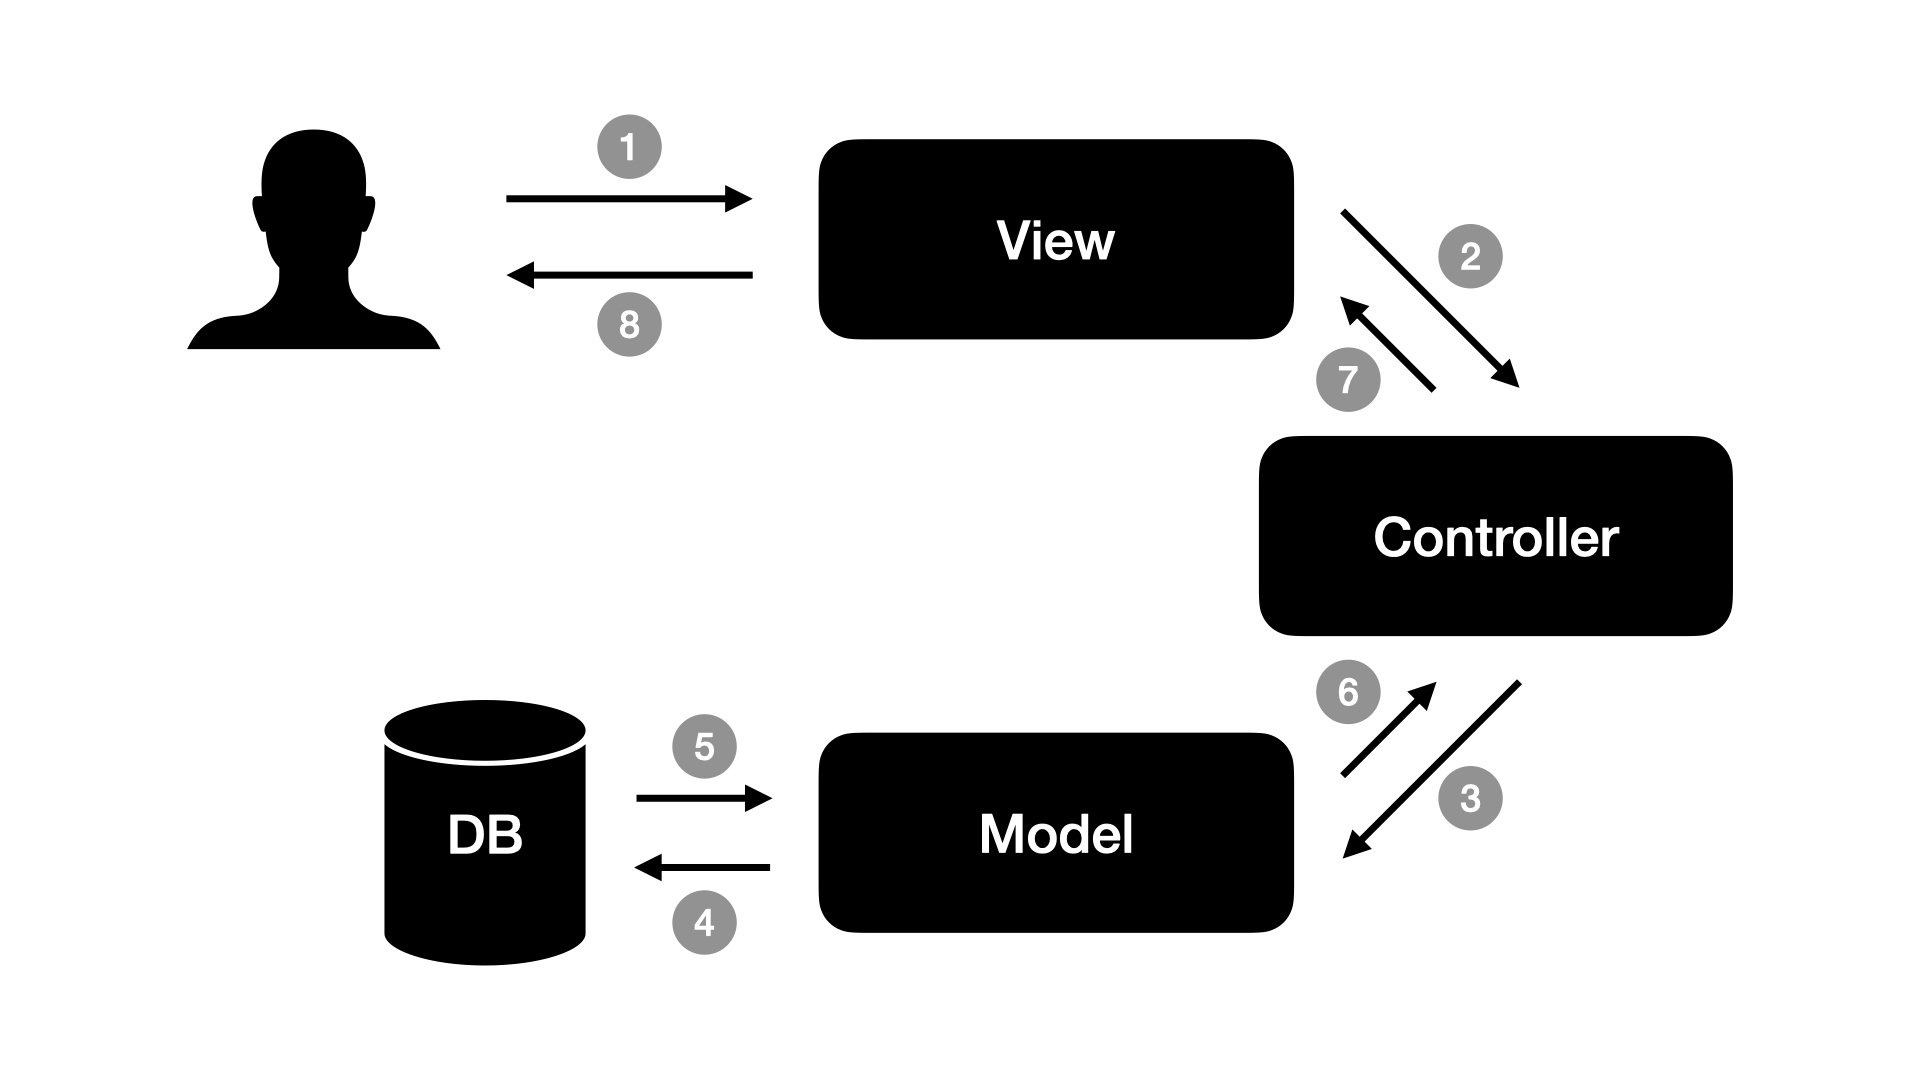
\includegraphics[width=.6\textwidth]{Assets/Interaktionsorientiert.001}
	\caption[Kommunikation zwischen Controller und Model]{Kommunikation zwischen Controller und Model, \\ (1) Der Benutzer sieht die graphische Darstellung und führt eine Aktion aus (2). Der Controller verarbeitet die Aktion und ruft über das Model Daten ab (3). Das Model greift auf die Datenbank zu und lädt die entsprechenden Informationen (4 und 5). Anschließend gibt das Model die Inhalte an den Controller zurück (6). Dieser gibt die Daten an die View weiter (7), welche abschließend die neuen Inhalte dem Benutzer anzeigt (8).}
	\label{fig:mvc-cm-kommunikation}
 \end{figure}
 
 \begin{figure}
 	\centering
    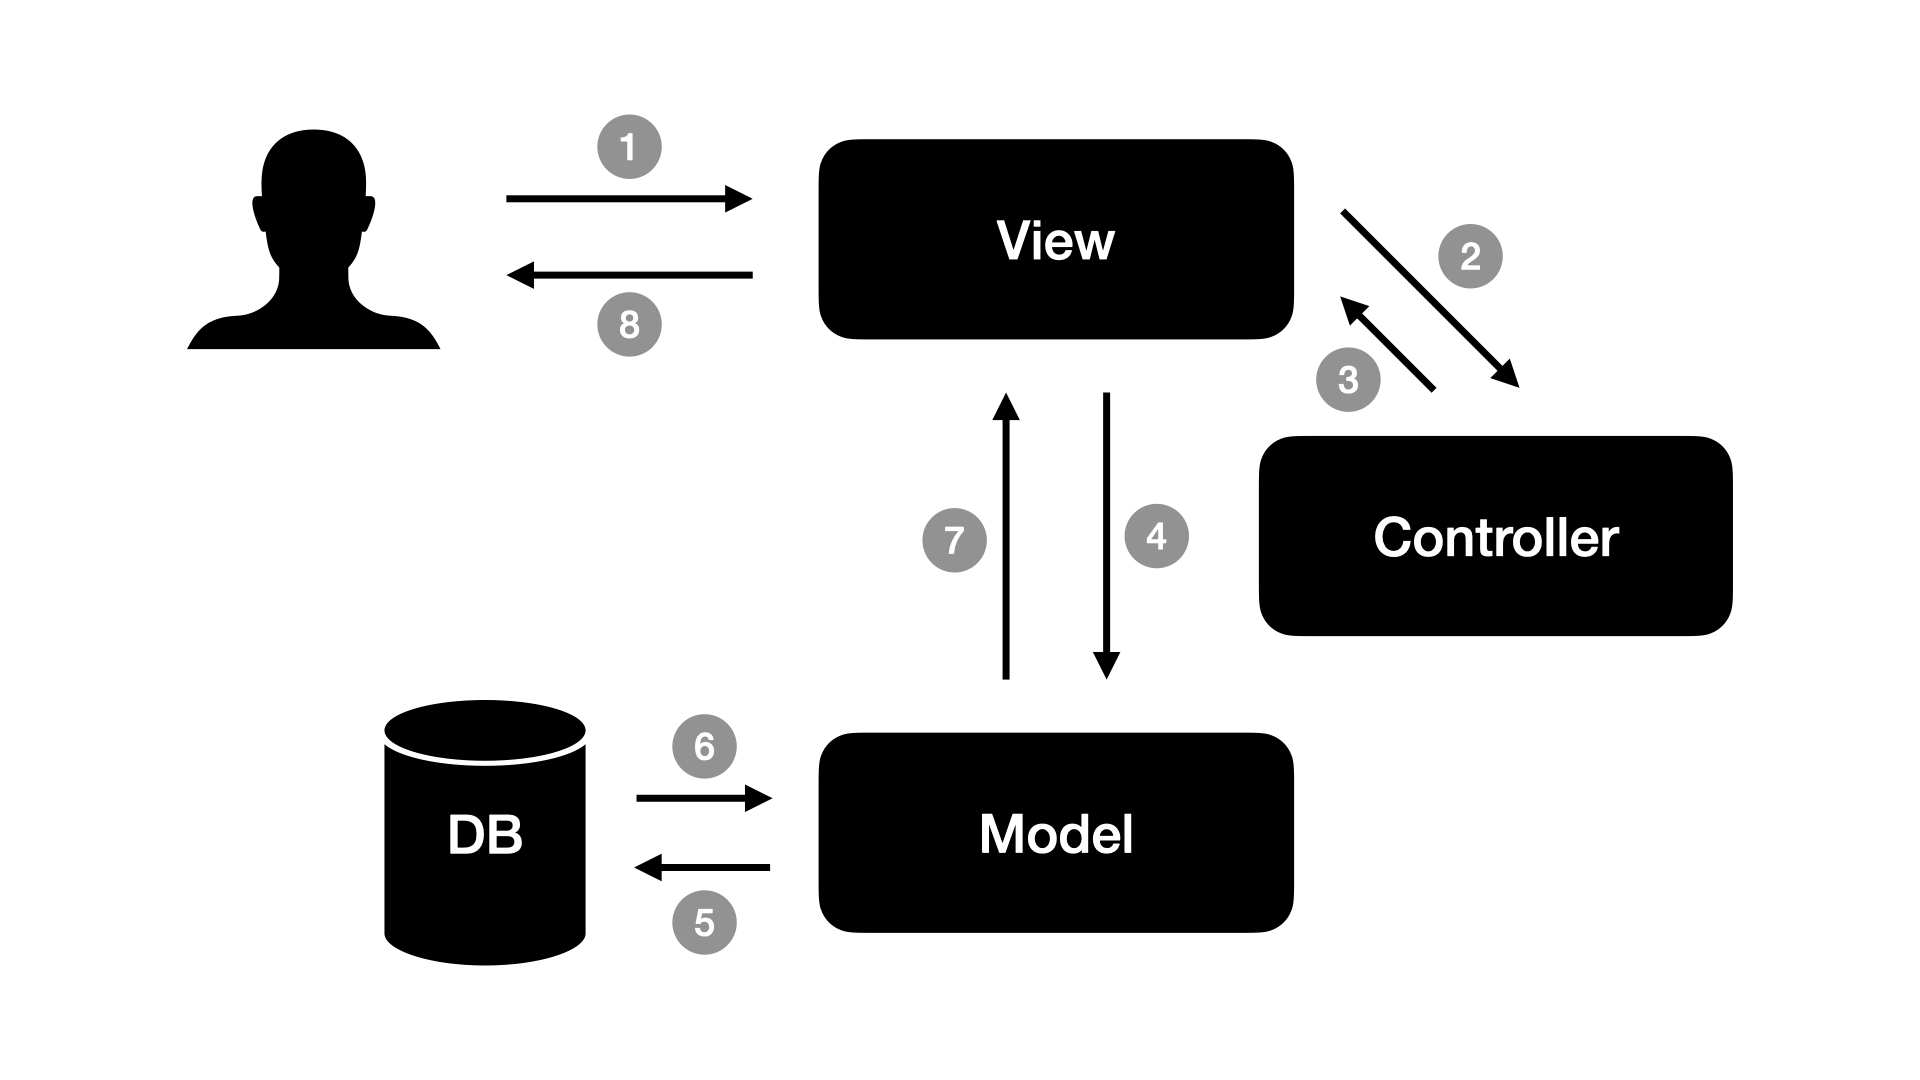
\includegraphics[width=.6\textwidth]{Assets/Interaktionsorientiert.002}
	\caption[Kommunikation zwischen View und Model]{Kommunikation zwischen View und Model, \\ (1) Der Benutzer sieht die graphische Darstellung und führt eine Aktion aus (2). Der Controller verarbeitet die Aktion und rendert umgehend die graphische Darstellung (3). Die View lädt über das Model die Daten (4). Das Model greift auf die Datenbank zu und lädt die angeforderten Informationen (5 und 6). Anschließend gibt es die Inhalte an die View zurück (7). Dieses zeigt abschließend die neuen Inhalte dem Benutzer anzeigt (8).}
    \label{fig:mvc-vm-kommunikation}
 \end{figure}

\subsubsection{REST-Architektur}
\label{sec:rest}

Neben den bislang genannten Architekturstilen, gibt es eine Vielzahl von weiteren Strukturierungen, die sich erst in den letzten 20 Jahre entwickelt haben. Einer dieser Architekturstile ist die REST-Architektur, welche vom Miterfinder des HTTP-Standards Roy Fielding definiert wurde \parencite[][S. 128]{starke_effektive_2015}. Er beschrieb diesen Stil in seiner Dissertation an der Universität von Kalifornien im Jahr 2000 und charakterisiert ihn als Architekturstil für das Web.

Dabei steht REST für \textit{Representational State Transfer}, welches einen Architekturstil für verteilte Systeme beschreibt und auf der Client-Server-Architektur aufbaut \parencite[][S. 76]{fielding_architectural_2000}. Client-Server-Architektur beschreibt eine Ausprägung eines verteilten Systems, bei dem die Anwendung in Server und Clients geteilt werden \parencite[][S. 117]{starke_effektive_2015}.\footnote{Dabei beziehen sich die Begriffe \textit{\enquote{Server}} und \textit{\enquote{Client}} auf Software Komponenten und auf den physischen Server und das Endgerät des Nutzers (Client). Des Weiteren grenzt sich der Architekturstil von der Mainframe Architektur ab, bei der über Terminals Anweisungen an einen Großrechner gestellt werden.}

Ein Server ist dabei eine Software Komponente im Netzwerk, welche Services anbietet. Ein Service könnte beispielsweise zuständig sein, alle Informationen der hinterlegten Kunden auszugeben. Der Client hingegen konsumiert lediglich diese Informationen und dient dem Benutzer als Bedienungsoberfläche. Dies bedeutet, dass der Server nur passiv auf Anfragen vom Client wartet, während der Client selbst keine Informationen verarbeitet, sondern ausschließlich anzeigt. Gleichwohl handelt es sich um ein Programm, welches auf dem Endgerät des Benutzers (Computer, Mobiltelefon) ausgeführt wird.

Die REST-Architektur verwendet diese Aufteilung, um eine feste Trennung der Zuständigkeit zu integrieren \parencite[vgl.][S. 78]{fielding_architectural_2000}.

Die zweite Bedingung, die Fielding an den Architekturstil stellt, ist dass die Kommunikation zustandslos, zu Englisch (stateless), abläuft \parencite[][S. 78]{fielding_architectural_2000}. Dies bedeutet, dass die Nachrichten, die zwischen Server und Client ausgetauscht werden, alle nötigen Informationen beinhalten \parencite[][S. 128]{starke_effektive_2015}. Somit gibt der Server auf Anfrage des Clients stets die gleiche Antwort zurück, egal ob dieser zum Ersten, oder zum wiederholten Mal angefragt wurde. Des Weiteren hängt die Antwort nicht vom Client ab.
Diese Entkopplung zwischen den Komponenten ermöglicht, dass die Aufgabe des Servers, sowie des Clients durch mehrere Computer verrichtet werden kann und  das System skalierbar ist \parencite[][S. 79]{fielding_architectural_2000}.

Der Hauptunterschied zwischen der REST-Architektur und anderen Stilen, liegt in der genauen Bestimmung der zu verwendenden Kommunikationsschnittstellen. So bestimmt die REST-Architektur sehr explizit, welche Form zur Kommunikation verwendet werden darf. So werden Methoden vom Server über HTTP-Standards aufgerufen. Konkret bedeutet dies, dass die einzelnen Dienste des Servers sich nach den HTTP-Methoden (GET, PUT, POST und DELETE) richten und es ein klares Mapping zwischen ihnen gibt. \parencite[vgl.][S. 128]{starke_effektive_2015}. Somit baut die REST-Architektur auf einem Kommunikationsstandard auf, der sich im Internet etabliert hat.

Auf Grundlage der standardisierten Kommunikation können zwischen Server und Client intelligente Zwischenstationen geschaltet werden, die dafür zuständig sind, häufig vorkommende Anfragen abzuspeichern \parencites[vgl.][S. 79 f.]{fielding_architectural_2000}[][S. 128]{starke_effektive_2015}.

Die Antwort des Servers erfolgt durch Repräsentationen der Daten, wovon es für jede Ressource\footnotemark mehrere Formate gibt. So kann eine Schnittstelle abhängig vom Aufruf sowohl JSON, als auch XML oder HTML zurückgeben \parencite[vgl.][S. 128]{starke_effektive_2015}.
\footnotetext{Als Ressource werden die Informationen bezeichnet, die durch den Aufruf einer URL zurück gegeben werden. Ein Beispiel wäre der HTTP-Aufruf \textit{GET: https://api.plurapolit.de/api/users}, der alle Informationen der User zurück sendet.}

Verwendet wird die REST-Architektur ausschließlich für Anwendungen im Internet, da es auf die Anwendung des Hypertext Transfer Protokoll\footnote{Weitere Informationen zum Hypertext Transfer Protokoll kann unter folgender Literatur gefunden werden \parencite{leach_hypertext_2020}.} (HTTP) angewiesen ist. Dabei findet der Architekturstil sowohl Anwendung für ganze Systeme, als auch in komplexen Anwendungen mit einer Vielzahl einzelner Services.

\subsubsection{Monolithische Architektur}
\label{sec:monolith}

Der Begriff \textit{\enquote{Monolith}} leitet sich vom altgriechischen \textit{\enquote{monólithos}} ab und bedeutet \textit{\enquote{aus einem Stein}} \parencites[vgl.][]{duden_nodate}[vgl.][]{dwds_nodate}. In der Gesteinskunde wird damit ein natürlich entstandener Gesteinsblock bezeichnet, der komplett aus einer Gesteinsart besteht \parencite[vgl.][]{dwds_nodate}.

Nach Rod Stephens liegt eine monolithische Softwarearchitektur vor, wenn jegliche Funktionalität des Systems miteinander verbunden ist. Dabei spricht er über die Verbindung von Dateneingabe, Datenausgabe, Datenverarbeitung, sowie Fehlerhandhabung und Benutzeroberflächen \parencite[vgl.][S. 94]{stephens_beginning_2015}.

Anders sieht es Sam Newman. Nach ihm liegt ein monolithisches System schon dann vor, wenn die gesamte Funktionalität eines Systems gemeinsam über einen Deployment-Prozess\footnotemark bereitgestellt wird \parencite[vgl.][Kap. 2.2]{newman_monolith_2019}. Folglich muss nicht zwingend jegliche Logik miteinander verbunden sein. Er unterteilt monolithische Systeme in drei Kategorien: Einzelprozess Monolithe, modulare Monolithe und verteilte Monolithe \parencite[vgl.][Kap. 2.2]{newman_monolith_2019}.
\footnotetext{Deployment-Prozess, oder auch Bereitstellungsprozess, bezeichnet den Prozess ein Software-System Benutzern zur verfügung zustellen \parencite[vgl.][]{softwareverteilung_2020}.}

Der Einzelprozess Monolith ist die gängigste Form und deckt sich mit der Definition von Rod Stephens. Es handelt sich dabei, um ein System bei dem das gesamte System einen Prozess abbildet. Dies bedeutet, dass jegliche Funktionalität aufeinander aufbauend ist und nur eine Datenspeicherung für die gesamte Anwendung verwendet wird \parencite[vgl.][Kap. 2.2.1]{newman_monolith_2019}.

Anders ist dies beim modularen Monolith. Er zeichnet sich darin aus, dass die Funktionalität in einzelne Module geteilt wird, die eine separate Datenspeicherung besitzen können \parencite[vgl.][Kap. 2.2.2]{newman_monolith_2019}. Im Gegensatz zu verteilten Systemen sind die einzelnen Module jedoch nicht auf separaten Computern verteilt, sondern über einen Rechner online gestellt. Des Weiteren sind die einzelnen Module nur leicht entkoppelt, sodass es zwischen ihnen Abhängigkeiten geben kann.

Dies ist bei verteilten Monolith anders, da die einzelnen Module komplett entkoppelt sind und Nachrichten ausschließlich über definierte Schnittstellen ausgetauscht werden \parencite[vgl.][S. 116]{starke_effektive_2015}. Ein verteilter Monolith erfüllt somit jegliche Anforderungen an ein verteiltes System mit der Ausnahme, dass alle Komponenten durch nur einen Prozess online gestellt werden.

Weder Stephens noch Newman geben Vorgaben hinsichtlich der Gliederung innerhalb eines monolithischen Systems. Demnach kann ein Model-View-Controller-Ansatz als monolithisches System gelten, solange es einheitlich bereitgestellt wird.

Im Rahmen dieser Arbeit wird beim Begriff Monolith stets von einem Einzelprozess Monolith ausgegangen, außer es wird expliziert von einem modularen, oder verteilten Monolithen geschrieben.

Vergleicht man das monolithische System mit einem verteilten System, gibt es Vor- und Nachteile \parencite[vgl.][Kap. 2.2.4 und Kap. 2.2.5]{newman_monolith_2019}. So ist das Bereitstellen eines Monoliths einfacher, da es einen Bereitstellungsprozess für die gesamte Anwendung gibt. Wiederum führt dies dazu, dass der Prozess deutlich länger dauert. Diese Tatsache ist besonders dann gravierend, wenn vermehrt kleine Änderungen vorgenommen werden. Andererseits vereinfacht eine Anwendung, die als ein Prozess zu sehen ist, die Fehlersuche und ermöglicht es Funktionen mehrfach zu verwenden. Das verursacht jedoch, dass schnell Abhängigkeiten entstehen können und Änderungen ungewollte Fehler verursachen. Dadurch wird die Umsetzung von neuen Funktionen mit steigender Codemenge verlangsamt und der Einstieg von neuen Teammitgliedern erschwert.

Da alle Entwickler eines Unternehmens auf einer Codebase arbeiten, kommt es schnell zu Unterschieden im Programmcode. So führt ein Monolith dazu, dass bei einer großen Anzahl von Entwicklern viele Absprachen notwendig sind \parencite[vgl.][Kap. 2.2.4]{newman_monolith_2019}.

Anders ist es bei systemübergreifenden Tests: Diese werden durch ein monolithisches System begünstigt und können im Vergleich zu einem verteilten System einfacher umgesetzt werden  \parencite[vgl.][Kap. 2.2.5]{newman_monolith_2019}.

\subsubsection{Einordnung des aktuellen Systems von PluraPolit}
\label{sec:einordnung}

Wie bereits in der Einleitung beschrieben, bietet PluraPolit eine Plattform an, die Jung- und Erstwählern bei der politischen Bildung unterstützt.

Es wurde ein Software-System entwickelt, welches auf der einen Seite PluraPolit die Möglichkeit gibt, Content zu verwaltet und auf der anderen Seite den Endkunden die Inhalte graphisch aufbereitet. Hierfür wurde, neben der Plattform für die Nutzer, ein Content Management System (CMS) umgesetzt. Programmiert wurde dieses in der Programmiersprache Ruby on Rails.\footnote{
Ruby on Rails, kurz auch als Rails bezeichnet, ist ein quellenoffenes Webframework, welches für die Programmiersprache Ruby entwickelt wurde \parencites[vgl.][S.4]{hartl_ruby_2016}{ruby_org}[vgl.][S. 24]{sieben_wochen}. Es ist komplett Open Source und wird von einer aktiven Community entwickelt. Es gibt eine Vielzahl von kostenfreien Paketen, sogenannte Gems, die nach Belieben zu einem Projekt hinzugefügt werden können. Im Vergleich zu anderen Frameworks zeichnet sich Rails besonders durch seine Implementierung der REST-Architektur aus \parencite[vgl.][S. 5]{hartl_ruby_2016}. Diese Implementierung führt jedoch dazu, dass eine Vielzahl von Bedingungen an die Entwicklung und Implementierung von Rails Anwendungen gestellt werden. Getreu dem Motto \textit{\enquote{Konvention vor Konfiguration}} nutzt Rails die Bestimmungen als Vorteil und integriert ein System, in das externe Pakete ohne Konfigurationsaufwand hinzugefügt werden können \parencite{ruby_doctrine}.
} Strukturiert werden Rails Anwendungen nach dem Model-View-Controller-Ansatz \parencites[vgl.][S. 66 ff.]{hartl_ruby_2016}.

\begin{figure}
	\centering
	\begin{subfigure}[a]{0.4\linewidth}
		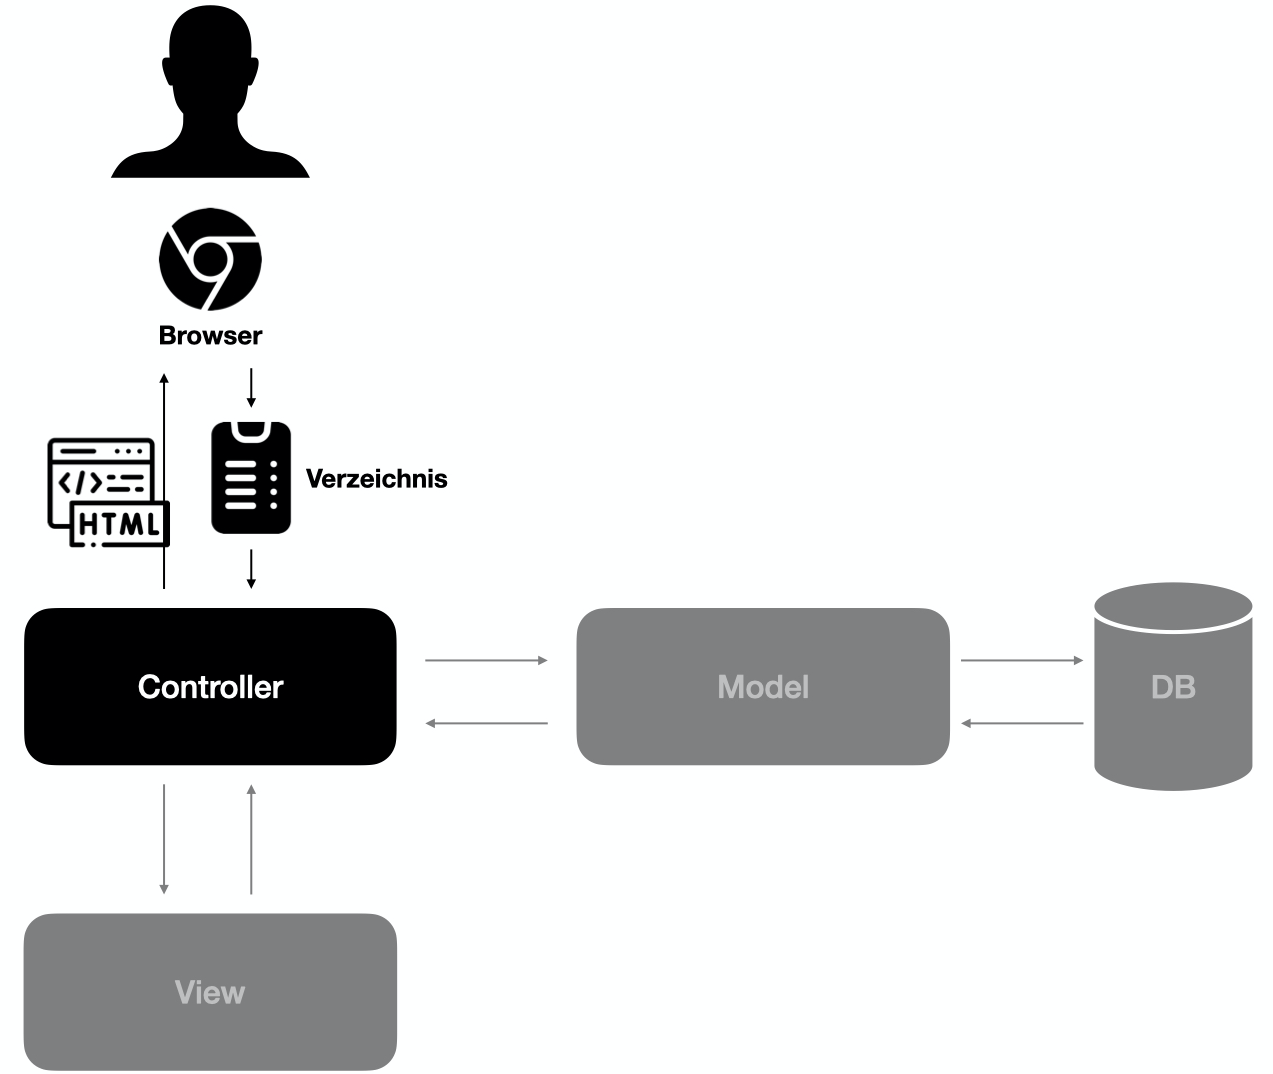
\includegraphics[width=\linewidth]{Assets/PluraPolit-Softwaresystem.001}
		\caption{Aufruf der Webseite}
		\label{fig:plurapolit-call-webpage}
	\end{subfigure}
	\begin{subfigure}[a]{0.4\linewidth}
		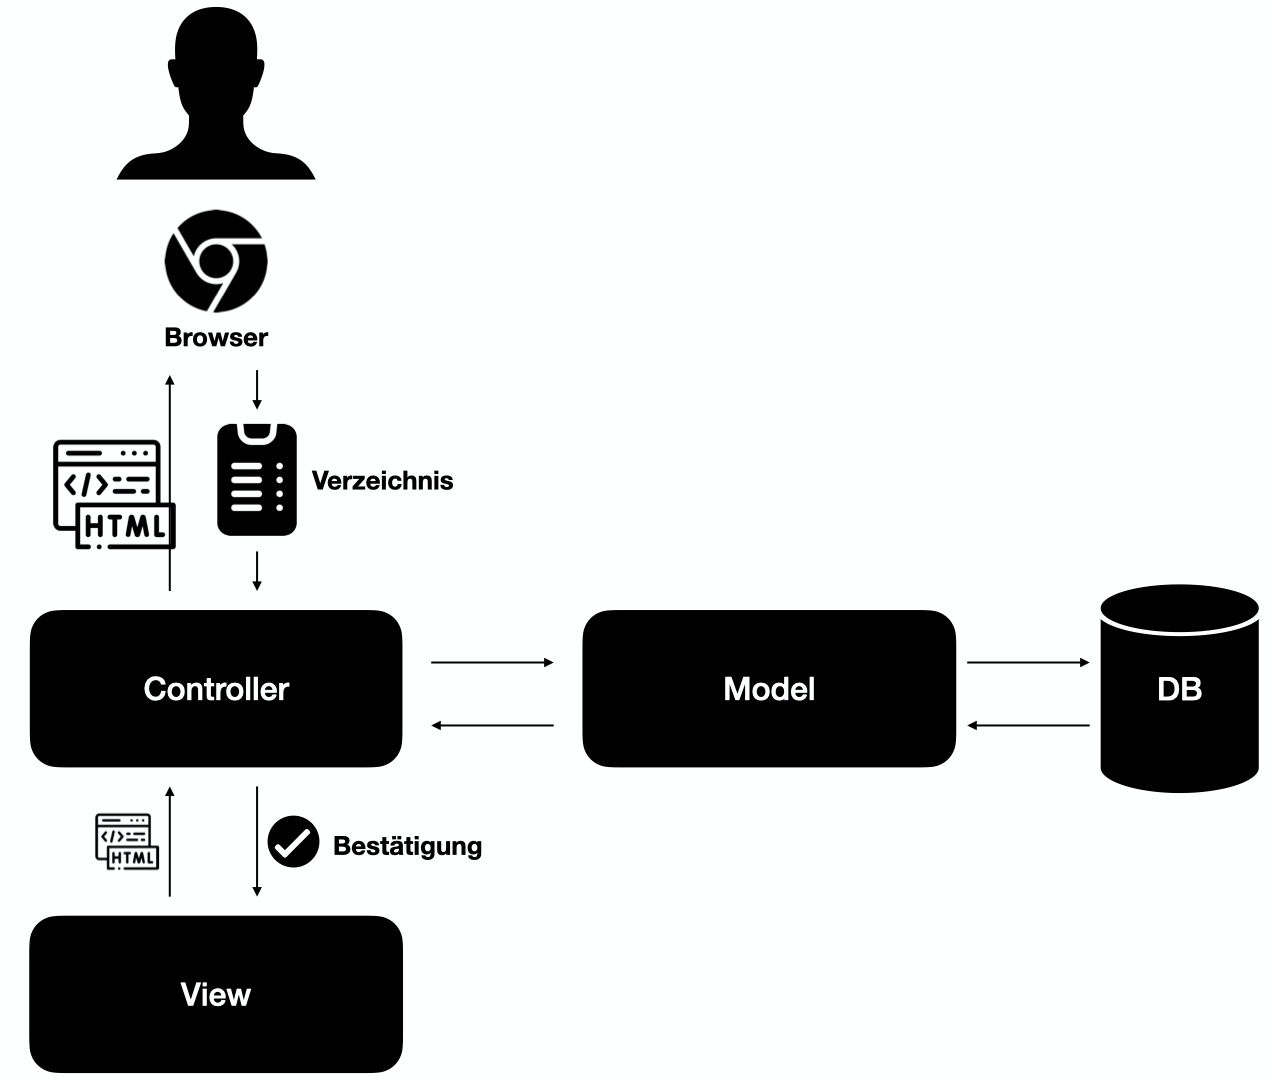
\includegraphics[width=\linewidth]{Assets/PluraPolit-Softwaresystem.002}
		\caption{Abspeichern der Tondatei}	
		\label{fig:plurapolit-save-sounddatei}
	\end{subfigure}
	\begin{subfigure}[b]{0.4\linewidth}
		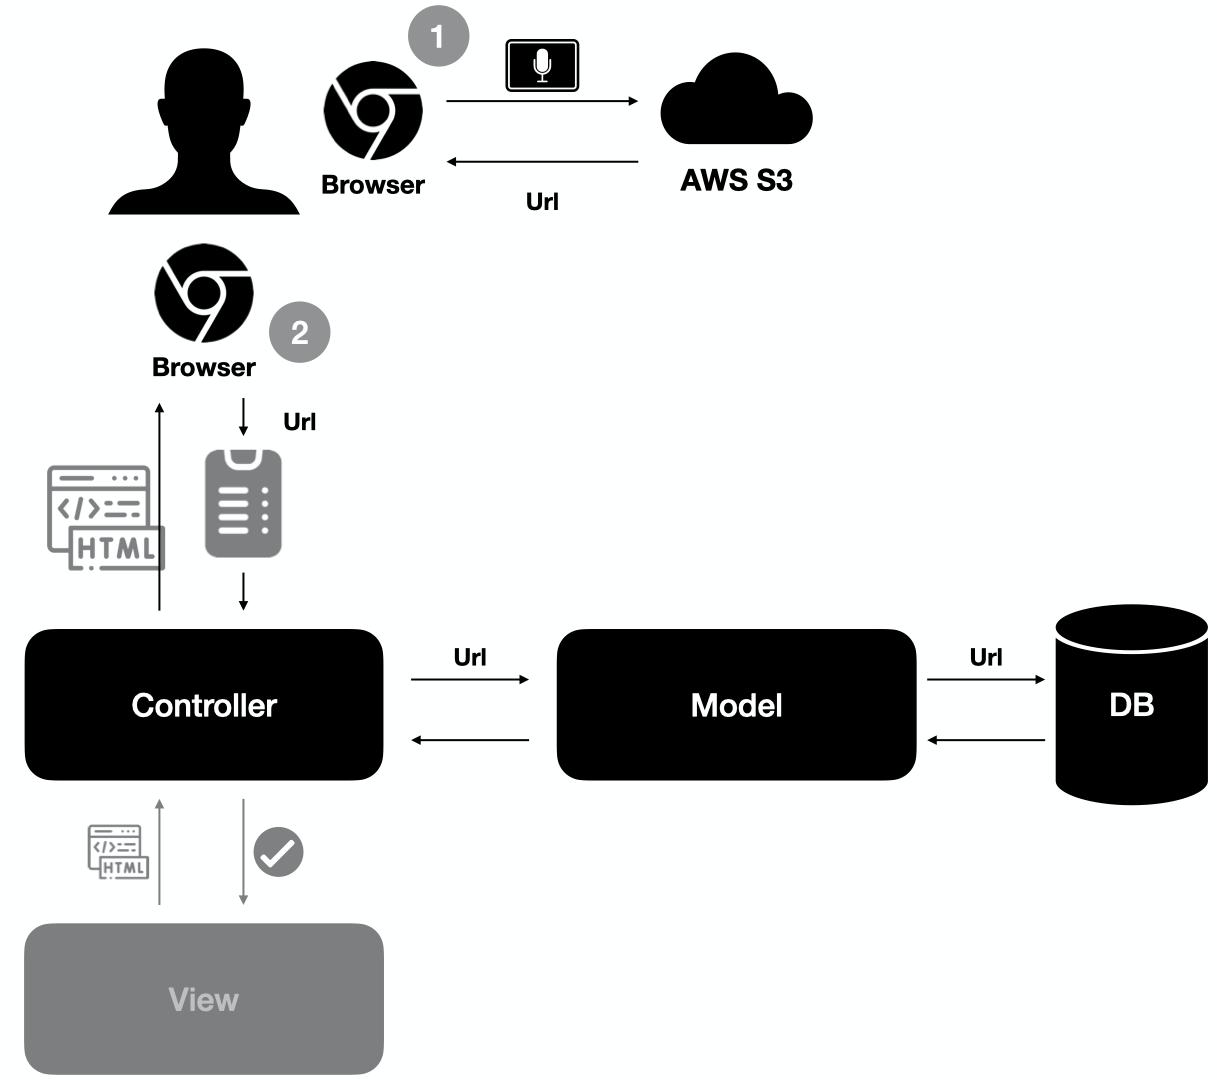
\includegraphics[width=\linewidth]{Assets/PluraPolit-Softwaresystem.003}
		\caption{Speichern zu S3}
		\label{fig:plurapolit-save-to-s3}
	\end{subfigure}
	\caption{Speichern einer Tonaufnahme}
	\label{fig:coffee}
\end{figure}

Um eine neue Tonaufnahme einzupflegen wird, die entsprechende Webseite im Browser aufgerufen. Dabei sendet der Browser über die URL eine Anfrage an den Server, der anhand eines Verzeichnis den verantwortlichen Controller bestimmt und die Anfrage an diesen weiterleitet.  Der Controller verarbeitet die Anfrage und schickt eine HTML-Seite zurück (siehe \cref{fig:plurapolit-call-webpage}).

Über diese Webseite kann die Aufnahme hochgeladen und abgespeichert werden. 
Dies geschieht, indem per Klick im CMS ein HTTP-Anfrage an den Controller geschickt wird. Der Controller speichert den Eintrag und bestätigt das erfolgreiche Abspeichern im View. Das Speichern geschieht dabei über das Model (siehe \cref{fig:plurapolit-save-sounddatei}).

Dabei wird die Tondatei selbst nicht in der Datenbank gespeichert, sondern lediglich ein Verweis darauf. 
Die Datei wird vorher zum Speicherservice von Amazon Web Services (S3) geladen, welcher die Tonaufnahme über eine URL zur Verfügung stellt. Nur die URL wird in die Datenbank hinterlegt (siehe \cref{fig:plurapolit-save-to-s3}).

\begin{figure}
	\centering
	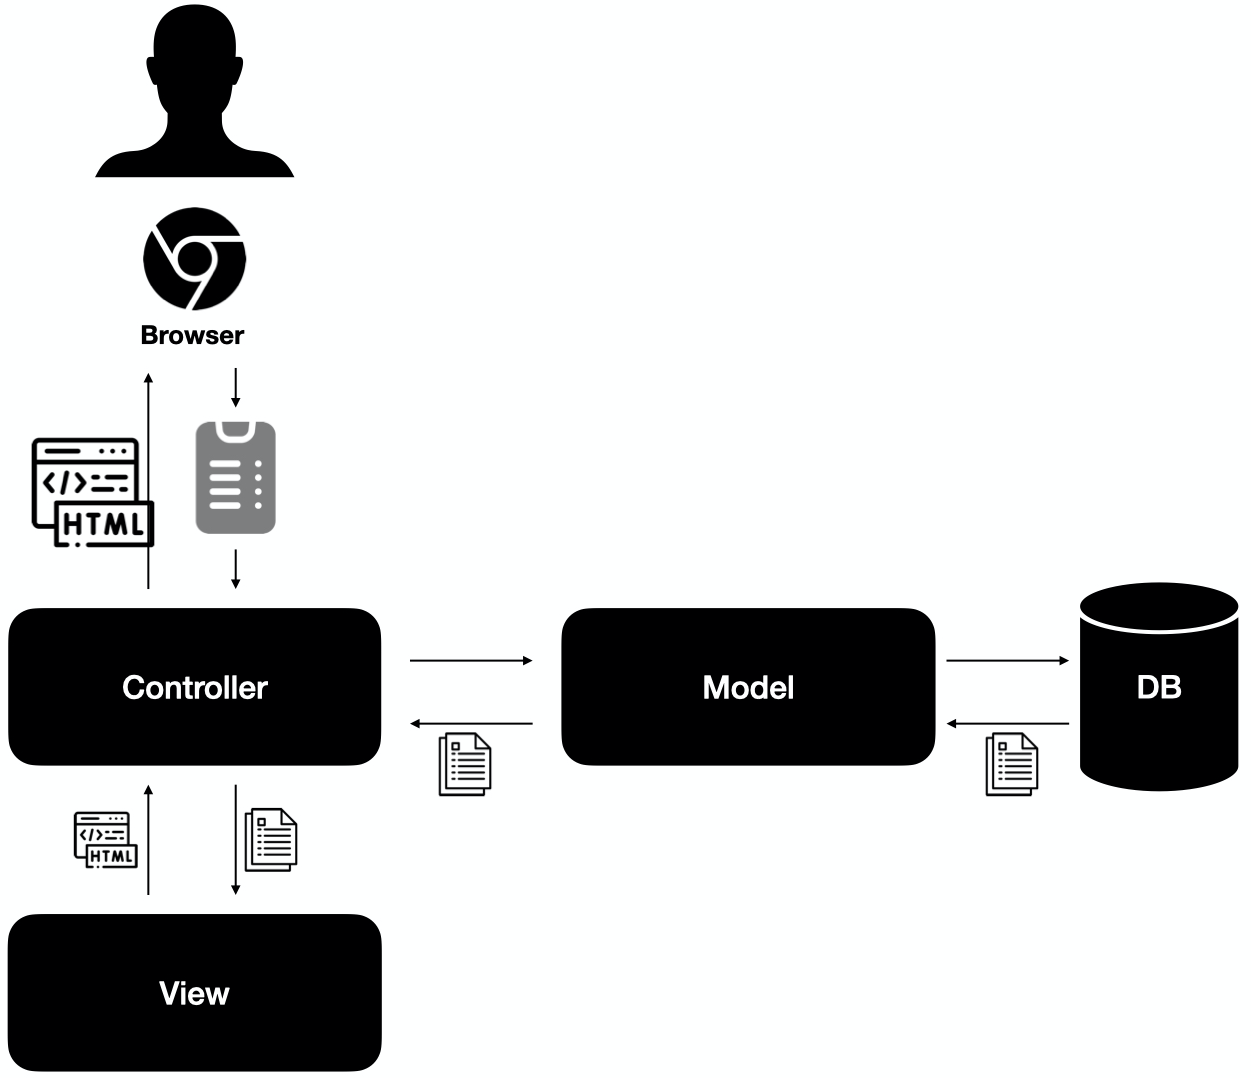
\includegraphics[width=0.5\linewidth]{Assets/PluraPolit-Softwaresystem.004}
	\caption{Inhalte bearbeiten}
	\label{fig:plurapolit-edit}
\end{figure}

Neben dem Abspeichern der Tonaufnahmen kann das CMS auch zum Bearbeiten und Anpassen von bestehenden Datensätzen genutzt werden. Hierfür wird die jeweilige Webseite aufgerufen, welches dazu führt, dass der Controller die angeforderten Daten aus der Datenbank lädt und die entsprechende graphische Darstellung an den Browser zurück gibt. Dabei greift der Controller nicht direkt auf die Datenbank zu, sondern lädt die Inhalte über den Model.
Auch übergibt der Controller lediglich die geladenen Inhalte an die View, welche  die Daten über Embedded RuBy in HTML integriert und die fertige Webseite  an den Controller zurück gibt (siehe \cref{fig:plurapolit-edit}).

\begin{figure}
	\centering
	\begin{subfigure}[c]{0.3\linewidth}
		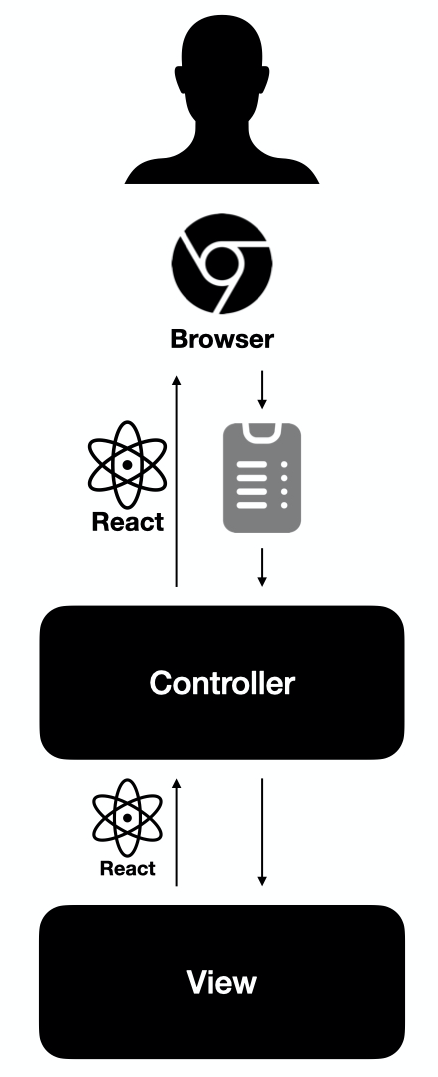
\includegraphics[,height=7cm]{Assets/PluraPolit-Softwaresystem.005}
		\caption{React-App aufrufen}
		\label{fig:plurapolit-load-react}
	\end{subfigure}
	\begin{subfigure}[c]{0.6\linewidth}
		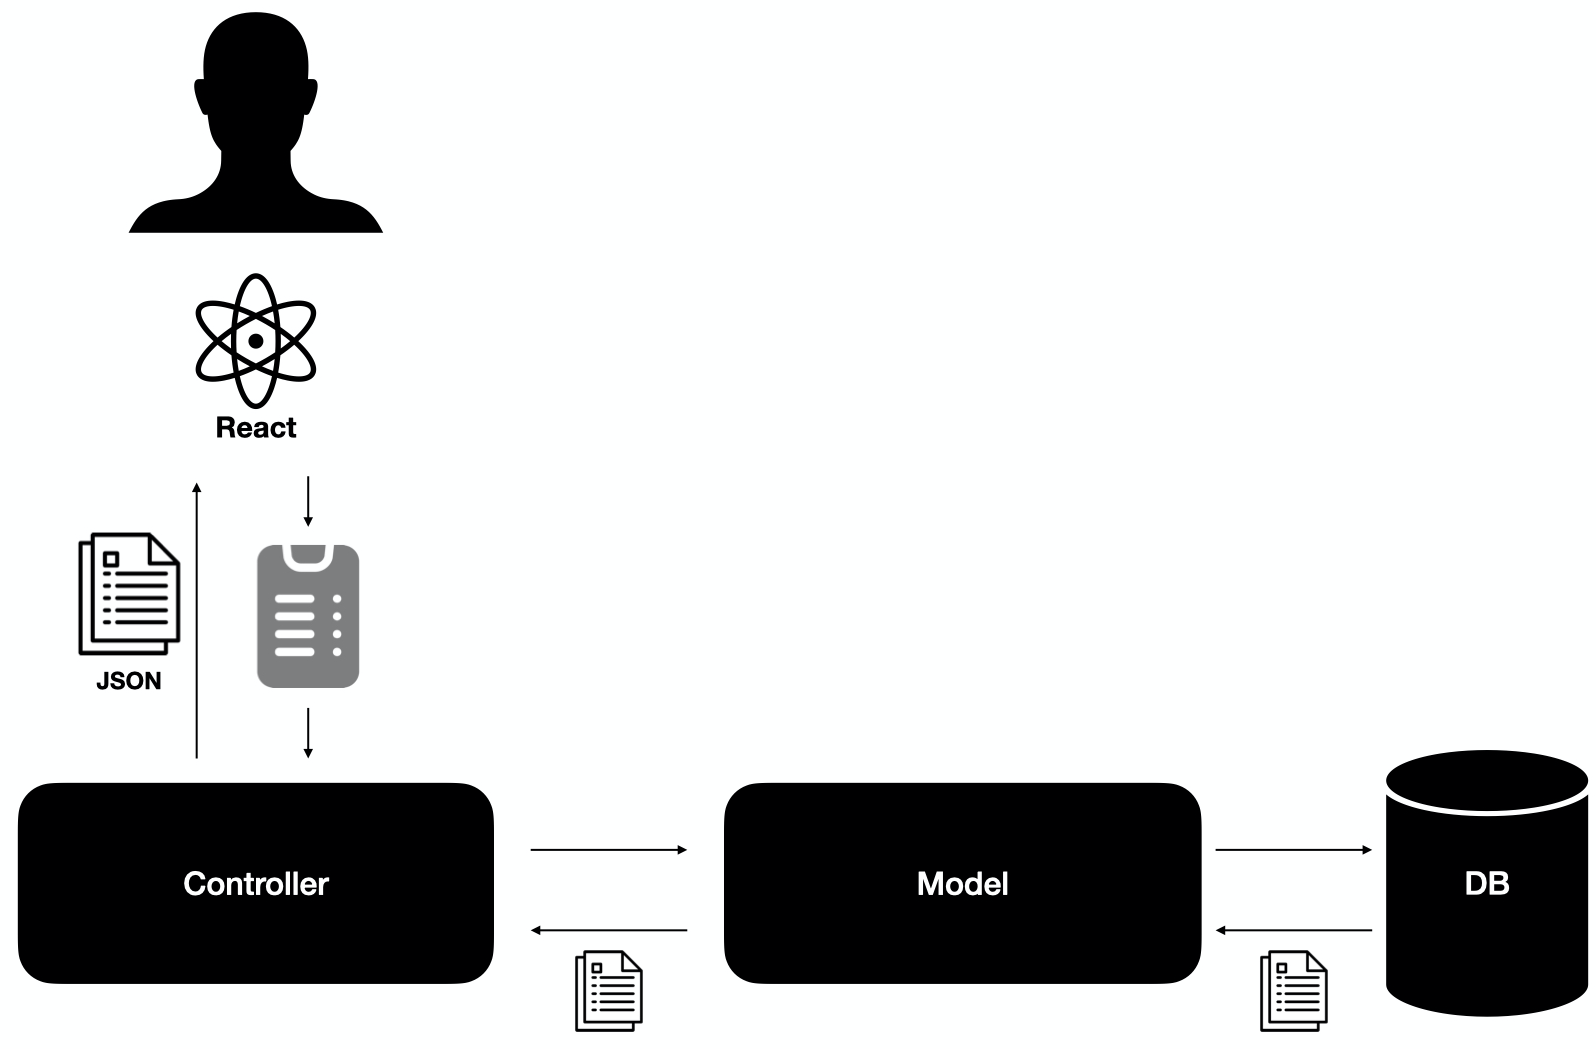
\includegraphics[width=\linewidth]{Assets/PluraPolit-Softwaresystem.006}
		\caption{React-App lädt Inhalte}
		\label{fig:plurapolit-react-data}
	\end{subfigure}
	\caption{Endkunde lädt die Plattform}
\end{figure}

Bei der Plattform für die Endkunden handelt es sich, um die selbe Anwendung wie beim CMS, mit dem Unterschied, dass die graphischen Darstellung durch eine React-Anwendung übernommen wird. So wird beim Aufruf der Plattform eine Anfrage an den Controller geschickt, der anschließend die kompilierte React-Anwendung zurück gibt (siehe \cref{fig:plurapolit-load-react}).

Diese lädt eigenständig jegliche Informationen über HTTP-Anfragen und kümmert sich um interne Seitenaufrufe. Die Anfragen werden dabei asynchron an die Rails Applikation geschickt und vom Controller beantwortet. Somit erhält die React-Anwendung über die Kommunikation von Controller und Modul, den Content aus der Datenbank, der vorher eingepflegt wurde (siehe \cref{fig:plurapolit-react-data}).

Es gibt also eine Aufteilung bezüglich der graphischen Darstellung in Content Management System und Plattform. Die Datenspeicherung und Verwaltung sind jedoch gleich. Die gesamte Codebase wird in einem Bereitstellungsprozesses dem Hosting Service zur Verfügung gestellt. Damit handelt es sich bei dem System von PluraPolit um ein Monolith, welches teilweise modular ist, die REST-Standards erfüllt und nach dem Model-View-Controller-Ansatz strukturiert ist. Des Weiteren nutz das System vereinzelt externe Services von AWS, um Tondateien zu speichern.


\subsection{Microservices}

Nachdem nun die einzelne Architekturstile vorgestellt wurden und das System von PluraPolit eingeordnet wurde, wird nun Microservices vorgestellt.

Dabei handelt es sich um eine Architekturstil, der ein Vertreter der verteilten Systeme ist und sich historisch aus der Service Orientierten Architektur abgeleitet hat (siehe \cref{sec:Zielsetzung}).

Eberhard Wolff beschreibt Microserivces als Ansatz Software in einzelne Module zu teilen und definiert es als Modularisierungskonzept, welches Einfluss auf die Unternehmesorganisation und Software-Entwicklungsprozess hat \parencite[vgl.][Kap. 1.1]{wolff_microservices_2018}. Dabei ist jedes Module ein eigenes Programm.

Sam Newman schließt sich Wolff an und beschreibt Microservices als voneinander unabhängig einsetzbare Dienste, die um eine Geschäftsdomäne herum modelliert sind \parencite[vgl.][Kap. 2.1]{newman_monolith_2019}.

Somit beschreiben beide Microservices als ein System aus einzelnen unabhängigen Services, die sich an ein Geschäftsdomäne richten. Insbesondere die Abhängigkeit zum Geschäftsprozess wird nachfolgend näher beschrieben.

\subsubsection{Zusammenhang und Verknüpfung}

Wenn es um das aufteilen von Software geht, ist es wichtig zu verstehen wie die einzelnen Funktionen und Klassen zusammenhängen und welche Verknüpfungen es zwischen ihnen gibt.

Dabei bezieht sich der Zusammenhang auf die funktionale Abhängigkeit zweier Funktionen oder Klassen \parencite[vgl.][Kap. 2.3.1]{newman_monolith_2019}. Somit liegt ein hoher Zusammenhang vor, wenn Quellcode anhand seiner logischen Zugehörigkeit geordnet ist. Eine konkrete Umsetzung dieses Bestreben ist im Abschnitt zum Model-View-Controller-Ansatz zu finden.

Verknüpfung hingegen beschreibt in welchem Maß, Funktionen und Klassen verbunden sind, ohne dass sie logisch zusammen gehören \parencite[vgl.][Kap. 2.3.2]{newman_monolith_2019}. Somit bezieht sich Verbindung ausschließlich auf eine technisch vorliegende Kopplung. Ein typisches Beispiel hier für ist, wenn ein Datenabruf an mehreren Stellen direkt über das Datenbankschema abläuft. Dadurch entsteht eine Abhängigkeit auf das Schema, sodass falls sich das Schema ändert auch die jeweiligen Aufrufe geändert werden müssen.

Insbesondere in monolithischen Systemen können viele Verknüpfungen entstehen, da keine festen Abgrenzungen zwischen einzelnen logischen Bereiche definiert sind. Somit kann es sein, dass ein Monolith, welches historisch wächst, keine klare Struktur aufzeigt. Es entsteht hieraus ein System, welches anfällig für Veränderungen ist.

Für ein Microservicesarchtektur ist jedoch das Bestreben klare Abgrenzung zu erlangen, und einzelne stabile Services zu etablieren. Diese sollen soweit es geht von einander entkoppelt funktionieren. Somit ist das Ziel für eine Microservicearchitektur einen hohen Zusammenhang bei geringer Verknüpfung zu besitzen. Dabei ist dies nicht nur die Zielsetzung für Microservices allgemein, sondern ein generelles Bestreben für stabile Systeme.\footnote{Dies bezieht sich auf das Gesetz von Constantine, welches besagt \textit{\enquote{A structure is stable if cohesion is strong and coupling is low.}} \parencite[S. 43]{endres_handbook_2003}.} Für Microservices bedeutet dies Konkret, dass ein Services ausschließlich aus funktional abhängigem Quellcode besteht und technische Implementierungen, wie zum Beispiel Datenbankstrukturen und Funktionsaufrufe, hinter klar definierten Schnittstellen versteckt sind.

\subsubsection{Conway's Law}

Die Abhängigkeit der Kommunikationsstruktur im Unternehmen zur verwendeten Software Architektur.

\begin{itemize}
	\item Begriff erklären
	\item Auswirkungen für die Teamstruktur beschreiben
\end{itemize}

\subsubsection{Bounded Contexts}

An diesem Punkt sollte eine Definition des Begriffes Bounded Contexts gegeben werden. Dies ist insbesondere wichtig, da Domain Driven Design darauf aufbaut und Bounded Contexts umsetzt.

\subsubsection{Domain Driven Design}

\begin{itemize}
	\item Was ist DDD?
	\item Was sind Bounded Contexts?
	\item 	Bespiele dazu.
	\item Schlussfolgerung für PluraPolit
\end{itemize}


\subsection{Microservice}

Wie aus dem vorhergehenden Abschnitt hervor geht sind Microservices einzelne, unabhängige Services, die um eine Geschäftsdomäne modelliert sind, welche auf Grundlage der klaren Schnittstellen entkoppelt und durch einzelne Kontext begrenzt sind. Die Kontexte ermöglichen das Verwenden von Service internen Terminologie und Verwendung ausschließlich benötigter Daten. Abschließend hat \cref{sec:conway} gezeigt, dass nur ein Team für ein Service zuständig ist.

In seinem Buch \textit{Monolith to Microservices} geht Newman darauf ein, dass wohl die wichtigste Eigenschaft von einem Microservice die unabhängige Einsetzbarkeit ist \parencite[vgl.][Kap. 2.1.1]{newman_monolith_2019}. Er sieht darin die Verkörperung von Unabhängigkeit und eigenständigen Teams, welche durch die Kommunikation der Services durch standardisierte Schnittstellen ermöglicht wird. Die meist verbreitete Art der Schnittstelle ist die nach dem REST-Standard, welche sich an eine Kommunikation über HTTP richtet (siehe \cref{sec:rest}).
 
Da viele Programmiersprachen den Informationsaustausch über HTTP ermöglichen, ist ein Microservice unabhängig einer bestimmten Technologie. Somit kann jedes Team eigenständig entscheiden, welche Programmiersprache sie verwenden wollen \parencite[vgl.][Kap. 1.2]{wolff_microservices_2018}. Dadurch können Sprachen nach Präferenz und Problemstellen gewählt werden, ohne dass eine Inkompatibilität zum Rest des Systems entsteht.

Vielmehr ermöglicht der Austausch über standardisierten Kommunikationswege, dass Services erstellt werden, die austauschbar sind \parencite[vgl.][Kap. 1.2]{wolff_microservices_2018}. Somit können zum Beispiel einige Services durch Dienste von Drittanbieter ausgeführt werden und Entwicklungskosten gespart werden. Außerdem wird dadurch die Möglichkeit geschaffen auf bestehender Logik aufzubauen und ältere Systeme mit modernen Technologien zu verbinden.

\cref{sec:ddd} hat gezeigt das Kontextgrenzen Microservices es ermöglicht Daten nach eigenem ermessen zu benennen und zu verwalten. Konkret besitzt jeder Dienst eine eigene Datenspeicherung, in Form zum Beispiel eines File-Storage-Systems oder einer Datenbank \parencite[vgl.][Kap. 2.1.3]{newman_monolith_2019}. Für das Gesamtsystem bedeutet dies, dass keine einheitliche Datenspeicherung vorliegt, sondern jeder Service die notwendigen Informationen verwaltet. Um jedoch die Funktionalität des gesamten Systems zu erhalten, müssen im Vorfeld bestimmt werden, wie der Informationsaustausch zwischen den Services abläuft \parencite[vgl.][Kap. 4.1]{wolff_microservices_2018}. Hierfür ist es wichtig zu bestimmen, welche Services welche Informationen verwalten und falls Abhängigkeiten zu anderen Diensten bestehen, die Schnittstellen festzulegen. Insbesondere die genauen Endpunkt und die zu erwarteten Informationen müssen bestimmt werden. Die Handhabung innerhalb eines Services, ist dann wieder dem einzelnem Team überlassen. 

Gibt es ein Service, der Informationen von einem anderen Dienst benötigt, fordert dieser die Daten über öffentliche Schnittstellen aktive an. Dies führt jedoch dazu, dass gleiche Informationen von mehrere Diensten verwaltet werden und es zu unterschieden Datenständen kommt \parencite[vgl.][Kap. 4.1]{wolff_microservices_2018}. Es entsteht die Herausforderung Informationen zwischen Services Konsistent zu halten (siehe \cref{sec:cap}).

Volle Unabhängigkeit eines Microservice kann nur erreicht werden, wenn dieser auch für die Benutzeroberfläche verantwortlich ist \parencite[vgl.][Kap. 4.4]{wolff_microservices_2018}. In der Praxis ist dies jedoch schwierig, da eine Webseite Inhalte von mehreren Services anzeigt. Insbesondere nachdem AngularJS\footnote{AngularJS ist ein JavaScript Framework, welches 2010 von Google entwickelt wurde und eine Open-Source-Software ist \parencite{angularjs}.} veröffentlicht wurde, gibt es immer mehr JavaScript Frameworks die um die Benutzererfahrung zu verbessern mehr Logik in das Frontend legen. React.js ist eines dieser Frameworks. Die Beliebtheit hinter diesen Frameworks, liegt darin, dass jede einzelne Webseite nicht mehr als einzelne Seite betrachtet wird, sondern Informationen zwischen Benutzeroberflächen hinweg verwaltet werden \parencite[vgl.][Kap. 9.1]{wolff_microservices_2018}. Dadurch kann ein Datenabruf über mehrere Webseiten geteilt werden und somit die Performance verbessern. Erreicht wird dies, indem das Routing zwischen den Webseiten durch das Framework verwaltet wird. Dieser Ansatz wird als Single-Page-Application (SPA) bezeichnet und unterscheidet sich von der Idee des Model-View-Controller aus \cref{sec:mvc}, da die nötigen Informationen aktive von der View geladen werden \parencite{single-page-webanwendung_2019}.

Da in der Praxis viele Webseiten Single-Page-Applicationen einsetzen, um eine gute Benutzererfahrung zu liefern, sollte in diesen Fällen über mögliche Teilung nachgedacht werden. Insbesondere wenn es sich um Applikationen handelt, die von mehrere Teams verwaltet werden. Ist dies nämlich der Fall, kann darunter die Unabhängigkeit der Teams leiden.

Auch kann es vorkommen, dass ein Microservices keine graphische Darstellung benötigt, da dieser zum Beispiel nur E-Mails verschickt oder die beliebtesten Filme ermittelt. Somit gibt es keine absolute Aussage darüber, ob ein Microservice eine Benutzeroberfläche haben sollte.

Insbesondere in puncto Skalierung bieten Microservices viele Vorteile \parencite[vgl.][Kap. 2.1.4]{newman_monolith_2019}. So lassen sich individuell, intensiv genutzte Services unabhängig vom Gesamtsystem skalieren. Dies kann ein großer Kostenvorteil sein, da nur ein einzelner Teil und nicht das gesamte System mehr Ressourcen zu geteilt werden muss. Auch können auf Basis der eingeteilten Teams weitere Entwickler angestellt werden und das Unternehmen hinsichtlich der Angestellten wachsen.

Während Microservices Skalierungen begünstigen, erschweren sie serviceübergreifende Veränderungen \parencite[vgl.][Kap. 2.15]{newman_monolith_2019}. Somit ist es auf Grund der technologischen Freiheit aufwendiger, Entwickler von einem Service zu einem Anderen zu überführen. Dies wird dadurch verstärkt, dass unterschiedliche Daten gespeichert und verschiedene Terminologien verwendet werden. Auch eine technologische Überführung von Funktionen wird erschwert, wenn verschiedene Programmiersprachen eingesetzt werden. Äquivalent ist das zusammenführen von Datenschemata, welches durch die unterschiedlichen Attributbezeichnungen boykottiert wird. Dies führt dazu, dass ein Zusammenschluss nur durch einen großen Aufwand erreicht werden kann.



\input{sections/Theory/produktmarketfit}

\subsection{Kommunikation von Services}
\label{sec:kommunikation}
%Todo Literatur einfügen

Aus \cref{sec:microservices} geht hervor, dass eine Microservice-Architektur aus einzelnen, unabhängigen Services besteht, welche voneinander entkoppelt sind. Um jedoch gleichzeitig die Funktionalität des Gesamtsystems zu gewährleisten, ist es notwendig, dass die einzelnen Services untereinander im Austausch stehen. Demzufolge stellt die Kommunikation eine Grundvoraussetzung für das Implementieren einer Microservice-Architektur dar und setzt voraus, dass ein Kommunikationsfähiges Netzwerk vorhanden ist.

Im Vergleich zu einem monolithen System hat jedoch der Austausch von einzelnen Services über ein Netzwerk einige Nachteile. So ist es Aufwendiger ein Systems aus einzelnen Komponenten richtig abzusichern, als ein einzelnen Rechner vor Angriffen zu schützen. Des Weiteren ist jede Schnittstelle, die öffentlich dem Netzwerk zur verfügung steht ein Risiko für potentielle Angriffe. Demzufolge erhöht die Umsetzung einer Microservice-Architektur die Gefahr für ein Angriff und ist gleichermaßen aufwendiger zu sichern. Anschließend ist der Aufruf über das Netzwerk langsamer und mit geringerer Bandbreite als ein Aufruf innerhalb eines Prozesses \parencite[vgl.][Kap. 6.1]{wolff_microservices_2018}.

Auch wenn bis lang nur auf die Kommunikation über den REST-Standard in dieser Ausarbeitung eingegangen wurde, ist es nicht die einzige Möglichkeit Schnittstellen zwischen Services zu definieren. So gibt es neben REST noch weitere Arten der Kommunikation, wie zum Beispiel GraphQL \parencite{graphql_docs} und gRPC \parencite{grpc_docs}. Beides sind Ansätze, welche in den letzten Fünf Jahren entwickelt wurden und deutlich andere Schwerpunkte setzen.

Im Unterschied zu REST muss bei GraphQL nicht für jeden Individuellen Client eine extra Schnittstelle geschrieben werden, sondern der Client gibt beim Aufruf die Informationen mit, welche er erhalten möchte \parencite[vgl.][]{graphql_docs}. Dabei wird im Vorfeld über ein Schema festgelegt, welche Informationen der Server zur Verfügung stellt. Auch können über GraphQL nicht nur Informationen von einer Relation (Tabelle) abgerufen werden, sondern über Verbindungen zwischen Relationen, auf Daten von anderen Tabellen zugegriffen werden. Auch hier wird die Spezifikation der Inhalte vom Client beim Aufrufen der Schnittstelle mitgegeben. Folglich entstehen wenige Programmschnittstellen, die jedoch eine Vielzahl Anforderungen bedienen können. Dies ist insbesondere für Aggregierte Informationen aus mehreren Tabellen wichtig, sowie für Systeme, in denen mehrere Clients unterschiedliche Informationen vom selben Service abrufen.

gRPC auf der anderen Seite ermöglicht es einem Client, Funktionen eines Servers übers Netzwerk aufzurufen, als währen sie in der gleichen Codebase. Hierbei ist gRPC Programmiersprachen unabhängig, sodass ein in Java geschriebener Client auf ein Python-Server zugreifen kann. Während REST explizit für Web-Anwendungen erstellt wurde, wurde gRPC speziell für den Austausch unter Services entwickelt. So werden zum Beispiel keine Statuscodes oder andere Meta-Daten verschickt, sodass die Geschwindigkeit im Vergleich zum REST-Standard schneller ist. Des Weiteren ermöglicht gRPC unteranderem das Monitoren der Kommunikation zwischen Services, um auftretende Fehler schnell erkennen zu können. Auch nutzt gRPC den moderneren HTTP/2 Standard, durch welchen der Datenaustausch beschleunigt und optimiert wird.

%Todo Noch einmal überprüfen, ob es wirklich 2003 war
Auch wenn 2003 Peter Rodgers Microservice-Architektur als ein System aus einzelnen REST-Services beschrieben hat, haben sich seitdem neue Technologien zur Kommunikation zwischen Services entwickelt. Insbesondere gRPC besitzt auf Grund der moderneren Technik bedeutende Vorteile hinsichtlich der Geschwindigkeit. Nichtsdestoweniger ist die Kommunikation zwischen entkoppelten Services langsamer, als Aufrufe innerhalb eines Prozesses und bringen einige Nachteile mit sich.

Demnach muss neben der Auswahl des Kommunikationsstandards ein Netzwerk vorliegen, welches einen hohen Durchsatz, als auch eine hohe Geschwindigkeit ermöglicht und vor Angriffe gesichert werden kann.


\subsection{Bedingungen ableiten}
\label{sec:bedingungen}

Aus den Erkenntnissen und Kernaussagen der vorangegangenen Abschnitte lassen sich Bedingungen ableiten, die als Leitfaden für die Entscheidungen von PluraPolit dienen. Im nächsten Gliederungspunkt werden diese von Experten qualitativ bewertet.

Wie in \cref{sec:conway} beschrieben, hat eine Microservice-Architektur das Ziel, Teams möglichst unabhängig voneinander arbeiten zu lassen. Erreicht wird dies, indem die Verantwortung eines Service nur einem Team übertragen wird und sich Absprachen zwischen den Teams auf die Festlegung der Schnittstellen begrenzen. Daraus ergeben sich zwei Bedingungen an das Unternehmen:
\begin{enumerate}
	\item Die Verantwortung für ein Geschäftsprozess muss an ein Team übergeben werden, und
	\item Die Services greifen ausschließlich auf Ressourcen zu, die über die Schnittstellen erreicht werden können.
\end{enumerate}

Der Abschnitt über Domain-Driven Design zeigt auf, dass Microservices die Komplexität eines Unternehmens reduzieren, indem die Geschäftsprozesse in Services aufgeteilt werden. Dieser Ansatz der Trennung der Geschäftsdomänen fördert die Fähigkeit, dass Services unabhängig voneinander wachsen können und gleichzeitig eine klare Verantwortung haben.

Es ergeben sich die Bedingungen zum Vorliegen eines Systems, welches:
\begin{enumerate}
	\item einerseits eine gewisse Komplexität aufweist und
	\item andererseits Geschäftsabläufe besitzt, die sich trennen lassen.
\end{enumerate}

Neben der Einteilung in einzelne Komponenten werden auch Bedingungen an das Netzwerk gestellt, wie in \cref{sec:kommunikation} ausgeführt. So ergeben sich folgende Anforderungen:
\begin{enumerate}
	\item Kommunikation der Services untereinander
	\item Verhinderung von unbefugten Zugriffen
	\item Vorliegen einer möglichst hohen Datengeschwindigkeit
\end{enumerate}

Wie in \cref{sec:kommunikation} vorausgesetzt, weisen die Services Programmierschnittstellen auf, die Server-zu-Server-Kommunikation erlauben.

Bei der Beschreibung der Situation eines Start-ups in \cref{sec:start-up} wurde deutlich, dass es in einem noch nicht existierenden Markt operiert und dadurch besonders dynamisch agieren muss. Daraus ergibt sich die Anforderung, dass erst eine Microservice-Architektur umgesetzt werden kann, wenn ein Product-Market Fit vorliegt.

Aus der Literaturrecherche ergeben sich zusammenfassend neun Bedingungen:
\begin{enumerate}
	\item Es ist möglich, die Verantwortung für ein Geschäftsprozess an ein eigenständiges Team zu geben.
	\item Die Services greifen ausschließlich auf Ressourcen zu, die über die Schnittstellen erreicht werden können.
	\item Das System weist eine gewisse Komplexität auf.
	\item Die Geschäftsabläufe lassen sich voneinander trennen.
	\item Das Netzwerk ermöglicht die Kommunikation zwischen den Services.
	\item Der Zugriff auf das Netzwerk ist vor Unbefugten gesichert.
	\item Das Netzwerk hat ein hohen Datendurchsatz.
	\item Die Services verfügen über Schnittstellen, die Server zu Server Kommunikation ermöglichen.
	\item Es liegt ein Product-Market Fit vor.
\end{enumerate}


\newpage

\section{Methodik}
\label{sec:methodik}

%Todo Text über das ermitteln der Bedingungen anhand der Literaturrecherche einfügen

Um herauszufinden, ob die Bedingungen aus der Literaturrecherche (\cref{sec:bedingungen}) notwendig sind, bevor PluraPolit seine Softwarearchitektur ändern kann, wurden Experteninterview durchgeführt. Es wurde sich für diese Methode entschieden, um trotz der wenigen Literatur, die es zu diesem Thema gibt, eine qualitative Einschätzung zu bekommen und abschließend eine Empfehlung für PluraPolit zu geben. Es wurde sich für ein Leitfadeninterview entschieden, um sowohl subjektive Erfahrungen zu erhalten, als auch die Antworten vergleichen zu können.

\subsection{Erstellung der Interviewfragen}

Die Fragen für die Interviews wurden aus den Ergebnissen der Literaturrecherche erstellt. So begann die Bachelor Thesis mit der Durchführung einer Literaturrecherche, in welcher Microservices und Softwarearchitektur definiert und beschrieben wurden. Nachfolgend wurden die zur Erstellung und Einteilung von Microservices notwendigen Faktoren benannt und beschrieben.  Die wichtigsten Inhalte wurden anschließend in \cref{sec:bedingungen} zu neun Bedingungen zusammengetragen und als Grundlage für die Fragestellung verwendet.

Dabei zielen die Fragen zum einen darauf ab, die einzelnen Annahmen zu validieren und zum anderen den Experten die Möglichkeit zu geben ihre Expertise einzubringen. Um dem gerecht zu werden, wurden vor allem offene Fragen gewählt. Gleichwohl orientierten sich die Fragestellungen an den in \cref{sec:bedingungen} definierten Bedingungen, sodass die Antworten aus den Interviews mit den Erkenntnissen aus der Literaturrecherche vergleichbar sind.

\subsection{Auswahl der Experten}

Für das Interview wurden Christoph Rahles, Alexander Troppmann und Sebastian Schlaak befragt.
Diese Experten wurden aufgrund ihrer jahrelangen Erfahrung im Bereich der Microservice-Architektur und Start-up-Branche ausgewählt. Sowohl Herr Rahles, Herr Troppmann und Herr Schlaak sind Senior Software Developer mit Erfahrungen im Management. So haben alle drei mehre Jahre als Chief Technology Officer (CTO) gearbeitet und können fundierte Aussagen über Software architektonische Entscheidungen geben. Darüber hinaus hält Herr Troppmann Informationsveranstaltungen in denen er erklärt, wie man mit Hilfe der Programmiersprache Golang leichtgewichtige Microservices erstellt kann.

Des Weiteren wurden alle drei ausgewählt, da sie PluraPolit kennen und bei der Entwicklung beteiligt waren. So hat Herr Rahles insbesondere in der Anfangsphase PluraPolit geholfen, die Softwarearchitektur mit aufzubauen und kennt diese detailliert.

Herr Troppmann und die Mitarbeiter von PluraPolit haben erst vor einigen Wochen gemeinsam an einem Hackathon teilgenommen und die Plattform konzeptionell weiter entwickelt. Es wurden Entwürfe erstellt, wie PluraPolit auch für den Schulunterricht eingesetzt werden kann. Folglich kennt Herr Troppmann den aktuellen Stand der Bildungsplattform.

Sowohl ich als auch Robin Zuschke haben vor der Zeit bei PluraPolit mit Herrn Schlaak zusammen gearbeitet und standen gelegentlich mit Herr Schlaak im Austausch. Demnach kannte Herr Schlaak vor dem Interview den technischen Standpunkt und die internen Abläufe.

Herr Rahles und Herr Schlaak kannten sich vor dem Interview, da sie von 2011 bis 2013 gemeinsam bei Käuferportal gearbeitet haben. Aufgrund dessen, dass die zwei Experten nach den gemeinsamen Arbeitsjahren in regelmäßigem Kontakt standen, wurden sie gebeten, sich nicht über die Inhalte des Interviews auszutauschen, sodass die Unabhängigkeit ihrer Antworten gewährleistet werden konnte.

Ausgenommen der Verbindung zwischen Herrn Rahles und Herrn Schlaak, kannten sich die Experten nicht.


\subsection{Durchführung des Interviews}

Die drei Experten wurden eine Woche vor dem Interview per Nachricht (Slack, oder WhatsApp) kontaktiert und zu einem Gespräch eingeladen, welches online stattfinden sollte. Es wurde ein Konferenzgespräch von Angesicht zu Angesicht gewählt, um eine persönlichere Atmosphäre zu generieren und gleichzeitig die Kontaktbeschränkungen in der Coronapandemie einzuhalten. Hinzu kam, dass Herr Troppmann in München wohnte und ein Gespräch nur online möglich war.

Alle Interviewpartner bekamen die Fragen zur Vorbereitung vorab zugeschickt. Sie wurden vor dem Gespräch in Kenntnis gesetzt, dass dieses aufgezeichnet wird, um die anschließende Transkripierung zu vereinfachen. Dies geschah zum einen während der Absprachen eine Woche vor den Interviews, sowie unmittelbar vor der Aufnahme. Des Weiteren gaben die Experten eine mündliche Bestätigung ab, dass ihre Aussagen in der Bachelorarbeit verwendet werden dürfen.

Um während des Interviews Rückfragen zu stellen, wurden zusätzlich zur laufenden Aufzeichnung kurze Notizen erstellt.

Die Interviews wurden nacheinander gehalten. Der erste Interviewpartner war Christoph Rahles am 18 Juni 2020 gehalten, gefolgt von Alexander Troppmann am 21 Juni und Sebastian Schlaak am 24 Juni.

In allen drei Fällen hat das Interview mit folgender Frage gestartet:

\textit{Haben Sie das Gefühl, dass es Bedingungen gibt, die PluraPolit erfüllen sollte, bevor es ihre Softwarearchitektur zu einer Microservice-Architektur umstellt und wenn ja, welche Bedingungen empfinden Sie als wichtig?}

Mit dieser Frage sollte die Annahme beantwortet werden, dass es überhaupt Bedingungen gibt. Weiterführend sollte den Experten die Möglichkeit gegeben werden, ohne jegliche Einschränkung notwendige Bedingungen zu nennen.

In zwei der drei Interviews (Christoph Rahles und Alexander Troppmann) wurden nach der ersten Frage die vierte Frage eingeschoben. Dies bot sich an, da beide Experten sich thematisch der besagten Fragestellung annäherten.

Es folgte Frage zwei:

\textit{Welche Rahmen Bedingungen sehen Sie als notwendig, dass Teams separat von einander Arbeiten können?}

Eingeleitet wurde diese Frage mit den Erkenntnissen aus der Literaturrecherche, dass Microservices es Teams ermöglichen, unabhängig von einander an unterschiedlichen Services zu arbeiten.

Diese Zusammenfassung sollte den Experten als Möglichkeit dienen, diese Annahme zu berichtigen und sich bei ihren Antworten darauf zu beziehen.

Die Frage zielte darauf ab, die Auffassung zu valideren, dass:
\begin{enumerate}
	\item Teams eigenverantwortlich arbeiten und
	\item ausschließlich über die Schnittstellen auf Informationen zu greifen.
\end{enumerate}
Es wurde sich für eine möglichst offene Frage entschieden, um den Experten die Möglichkeit zugeben, uneingeschränkt zu antworten.

Anschließend wurde Frage drei gestellt:

\textit{Gibt es in Ihren Augen irgendwelche technischen Anforderungen, die PluraPolit erfüllen sollte? }

Frage drei zielte darauf ab, Bedingung fünf, sechs und sieben zu überprüfen (siehe \cref{sec:bedingungen}). Demnach wurde erwartet, dass ein Netzwerk: 

\begin{enumerate}
	\item die Kommunikation zwischen den Services ermöglicht,
	\item Zugriffe verwaltet und
	\item ein hohen Datendurchsatz besitzt.
\end{enumerate}

Auch hier wählte man bewusst eine offene Fragestellung.

Frage vier ging der Fragestellung nach, ob Microservices in einem dynamischen Umgeld eingesetzt werden sollten. Hierfür wurde vorab eine Zusammenfassung aus der Literaturrecherche eingeschoben:

\textit{Ein Start-up zeichnet sich dadurch aus, dass es insbesondere in der Anfangsphase zu vielen Veränderungen in der ursprünglichen Geschäftsidee kommt. Microservices auf der anderen Seite zeichnen sich durch aus, dass sie feste Schnittstellen und Kontextgrenzen besitzen.}

Die Zusammenfassung sollte den Schwerpunkt der Fragestellung auf die Phasen eines Start-up lenken. Das Ziel dieser Frage war es, den Zeitpunkt, oder das Ereignis zu ermitteln, ab wann ein Start-up Microservices verwenden sollte. Ging der Experte nicht von selbst auf diese Fragestellung ein, gab es zusätzliche Fragen im Interview.

Abschließend wurde das Interview mit folgender Frage beendet:

\textit{Mit Ihrem aktuellen Wissensstand, welche Softwarearchitektur empfehlen Sie PluraPolit?}

Es wurde sich für diese Frage entschieden, um die Antworten mit den Antworten der vorhergehenden Fragen auf Einheitlichkeit zu überprüft und eine Einschätzung für PluraPolit zu geben.


\subsection{Methodik zur Auswertung}

Um die Interviews zu transkribieren, wurde der Dient \textit{Amazon Transcribe} von Amazon Web Services verwendet. Es handelt sich bei um ein Service, der automatisch, Audioaufzeichnungen in Text, konvertiert und diesen zurück gibt.

Nach dem automatischen Transkribieren wurden die Texte noch einmal korrigiert und überprüft.

Die einzelnen Aussagen aus den Interviews wurden offen codiert und anschließend in Themen zusammengefasst. Darauf folgend wurden diese Themen einzelnen Kategorien zugeordnet und sie weiterführend besser vergleichen zu können.

Abschließend wurden die Informationen aus den Interviews mit den Ergebnissen der Literaturrecherche verglichen und zu Erkenntnissen zusammengefasst. Mit Hilfe dieser Erkenntnissen wurde abschließend die Forschungsfrage beantwortet.


\subsection{Ergebnisse der Interviews}

\subsubsection{Frage 1}
\label{sec:frage1}

\textit{Haben Sie das Gefühl, dass es Bedingungen gibt, die PluraPolit erfüllen sollte, bevor es ihre Softwarearchitektur zu einer Microservice-Architektur umstellt und wenn ja, welche Bedingungen empfinden Sie als wichtig?}

Alle drei Experten beantworteten diese Frage mit Ja und nannten weitere Bedingungen (siehe \combref{appendix:r-1}, \combref{appendix:t-1} und \combref{appendix:s-1}).

Sowohl Sebastian Schlaak, als auch Alexander Troppmann gaben als Antwort an, dass sie erst Microservices in betracht ziehen, wenn inhaltlich unterschiedliche Anwendungen vorliegen. Herr Schlaak beschrieb in seinem Interview: \textit{\enquote{ich glaube, das wäre eine Bedingung, wenn man sagt: […] ich habe etwas [eine neue Funktion], was […] einen ganz anderen Zweck erfüllt […].}} (siehe \combref{appendix:s-5}). Herr Troppmann fasste es in seinem Interview wie folgt zusammen:  \textit{\enquote{Also wie gesagt, ich brauche eine technische Trennung […]}} und verwies auf die Trennung zwischen unterschiedlichen logischen Abläufen (siehe \combref{appendix:t-1}).

Als zweite Bedingung nannten die Experten die Wirtschaftlichkeit. Diese wurde  von Christoph Rahles und Alexander Troppmann hervorgehoben. Herr Rahles führte in seinem Interview an, dass es jemanden geben muss, \textit{\enquote{der […] sich die Frage stellt: Ist es wirtschaftlich, ja oder nein?}} (siehe \combref{appendix:r-3}). Herr Troppmann beurteilte es wie folgt: \textit{\enquote{[…] ich muss einen Business Case haben, [...][damit] sich das auch lohnt.}} (siehe \combref{appendix:t-2}). Daraus kann geschlussfolgert werden, dass der wirtschaftliche Nutzen eine wesentliche Voraussetzung für den Einsatz von Microservices ist.

Allein Herr Rahles verwies darauf, dass die Entscheidung für Microservices vom “Reifegrad des Geschäftsmodells” abhängt (siehe \combref{appendix:r-1}).


\subsubsection{Frage 2}

\textit{Microservices ermöglicht es Team unabhängig von einander an unterschiedlichen Services zu arbeiten. Welche Rahmen Bedingungen sehen Sie als notwendig, dass Teams separat voneinander Arbeiten können?}

%Todo Kommasetzung in der Frage überprüfen

Herr Rahles fügte den Vermerk hinzu, dass die Teams stets zu einem Unternehmen gehören und nie ganz unabhängig sind.\footnote{
\textit{\enquote{Auch diese Teams gehören zu einem Unternehmen […], das heißt unabhängig voneinander sind sie nie.}} (siehe \combref{appendix:r-15})
}

Herr Schlaak und Herr Troppman führten an, dass insbesondere Schnittstellen definiert und beschrieben sein müssen.\footnote{
\textit{\enquote{Ganz wichtig ist, dass die Schnittstellen der Services entsprechend gut beschrieben sind […]}} (siehe \combref{appendix:s-13}); \textit{\enquote{[…] die Teams müssen sich einig sein, über welche Schnittstelle die Services kommunizieren.}} (siehe \combref{appendix:t-19}); \textit{\enquote{Schnittstellen nach außen müssen geklärt sein.}} ( siehe \combref{appendix:t-22})
}

Weiterführend wurde von Herr Troppman eine Struktur hervorgehoben, die Abläufe genauer beschreibt.\footnote{
\textit{\enquote{[…] zumindest benötigt man Strukturen, sodass man weiß, was wie abläuft.}} (siehe \combref{appendix:t-22})
} Diesen Ansatz erwähnte auch Herr Rahles, als er die Notwendigkeit von Projektmanagement ansprach.\footnote{
\textit{\enquote{[…] es ist einfach sinnvoll zu gucken, dass […] die Teams entsprechend des Projektmanagements richtig aufgestellt sind.}} (siehe \combref{appendix:r-22})
} Daraus lässt sich folgern, dass Struktur notwendig ist, damit Teams separat arbeiten können.


\subsubsection{Frage 3}
\label{sec:frage3}

\textit{Gibt es in Ihren Augen irgendwelche technischen Anforderungen, die PluraPolit erfüllen sollte?}

Als wichtigste technische Anforderung stellte sich das Monitoring heraus. So beschrieben alle drei Experten die Notwendigkeit ein Monitoring zu implementieren, welches die Kommunikation zwischen den Services überwacht (siehe \combref{appendix:t-32} und \combref{appendix:s-16}). Besonders Herr Rahles verwies auf diese Bedingung.\footnote{
\textit{\enquote{Monitoring ist das A und O. Das heißt mit Anstieg der Komplexität, muss ich sicher sein, dass ich auch diese Komplexität hinreichend überblicken kann.}} (siehe \combref{appendix:r-31})
}

Auch die Sicherheit wurde von Herrn Rahles angemerkt. Dabei sah er es aber als Grundvoraussetzung für jegliche Infrastruktur und nicht explizit für Microservices.\footnote{
\textit{\enquote{Sicherheit gehört für mich zu den Grundvoraussetzungen, egal über welche Architektur wir reden.}} (siehe \combref{appendix:r-32})
}

Herr Schlaak und Herr Rahles hoben ein gut eingebautes Fehlermanagement hervor. So beschrieben beide, dass Services \textit{\enquote{vernünftige Fehlermeldungen}} zurück geben sollten (siehe \combref{appendix:s-18} und \combref{appendix:r-34}).

Aus den technischen Anforderungen Monitoring, Sicherheit und Fehlermanagement geht hervor, dass Kenntnisse in der Implementierung und in der Verwaltung der Infrastruktur vorhanden sein müssen. Eine Aussage, die auch von Herrn Troppmann bestätigt wurde.\footnote{
\textit{\enquote{[…] es [braucht] einen Entwickler, der sich mit dem Aufbau der Infrastruktur auskennt.}} (siehe \combref{appendix:t-33})
}

Herr Rahles bestärkte ebenfalls diese Schlussfolgerung, indem er die \textit{\enquote{heutzutage geltenden Best Practices als Anforderung}} nannte (siehe \combref{appendix:r-26}). Er führte diese Bedingung noch weiter aus und zählte automatische Tests, sowie einen automatischen Integration- und Deployment-Prozess zu den erforderlich Maßnamen (siehe \combref{appendix:r-27}).


\subsubsection{Frage 4}

\textit{Ein Start-up zeichnet sich dadurch aus, dass es insbesondere in der Anfangsphase zu vielen Veränderungen in der ursprünglichen Geschäftsidee kommt. Microservices auf der anderen Seite zeichnen sich durch aus, dass sie feste Schnittstellen und Kontextgrenzen besitzen. Meinen Sie, dass trotzdem Microservices in einem dynamischen Umfeld eingesetzt werden sollten?}

Christoph Rahles antwortete auf diese Frage, \textit{\enquote{Da gibt es glaube ich kein Richtig oder Falsch.}} und verdeutlichte, dass die Frage immer im Kontext der wirtschaftlichen und technologischen Lage des Start-up getroffen werden muss ( siehe \combref{appendix:r-6}).

Alexander Troppman vertrat die Meinung, dass Microservices grade im dynamischen Umfeld eingesetzt werden sollten. So gab er an, dass Microservices auf Grund des einfachen austauschen von Services im dynamischen Umfeld Sinn ergeben.
\textit{\enquote{Ich kenne viele Start-ups, die von Anfang an Microservices eingesetzt haben, weil grade Microservices so sind, dass man verschiedene Services austauschen kann. Also grade im dynamischen Umfeld machen Microservices Sinn.}} (siehe \combref{appendix:t-5})

Sebastian Schlaak antwortete, dass er mit einem Monolithen anfangen würde, da man dadurch deutlich schneller ist und führte weiter fort, dass die Vorteile von Microservices \textit{\enquote{erst in der späteren Skalierungsphase […] so richtig zum tragen kommen}} (siehe \combref{appendix:s-21}).

Die Aussage, dass man mit einem Monolithen anfängt, wurde von Herr Rahles bekräftigt. So äußerte er sich, \textit{\enquote{dass man [meistens] mit einem Monolithen anfängt}} und später, wenn \textit{\enquote{es sehr drückend wird}}, umstellt (siehe \combref{appendix:r-8}).

Herr Troppman bestärkt die Aussage, dass die Vorteile von Microservices erst später zum tragen kommen, indem er in seinem Interview sagte, dass eine Umstellung zu Microservices \textit{\enquote{sich erst mittel bis langfristig [lohnt]}} (siehe \combref{appendix:t-13}).

Sowohl Herr Rahles, als auch Herr Troppman antworteten, dass die Unternehmensziele die Entscheidung zur Umstellung beeinflussen. So verdeutliche Herr Rahles, dass die Entscheidung auch von der \textit{\enquote{Strategie der Firma}} abhängt (siehe \combref{appendix:r-12}).

Nach Herrn Schlaak sollte besonders, dann über eine Microservicearchitektur nachgedacht werden, wenn neue \textit{\enquote{Funktionen […] nichts mehr mit dem Kerngeschäft zu tun haben […]}} (siehe \combref{appendix:s-25}). Diese Aussage wird von Christoph Rahles geteilt. \textit{\enquote{Meistens ist es so, dass man mit einem Monolithen anfängt und irgendwann an ein Punkt kommt, […] wo man sagt, es macht Sinn Dinge auszulagern.}} (siehe \combref{appendix:r-9}).

%Todo Einfügen der Schlussfolgerung, dass die Entscheidung von der Komplexität der Geschäftsprozesse abhängt. GGf. anderes Wort für Komplexität.


\subsubsection{Frage 5}
\label{sec:frage5}

\textit{Mit Ihrem aktuellen Wissensstand, welche Softwarearchitektur empfehlen Sie PluraPolit?}

Alle drei Experten empfolen einen Monolithen (siehe \combref{appendix:r-38}, \combref{appendix:t-36} und \combref{appendix:s-31}).

Alexander Troppmann und Sebastian Schlaak haben weiterführend geraten, das Backend und das Frontend voneinander zu trennen. Herr Schlaaks Vorschlag war es, im Frontend ein \textit{\enquote{modernes JavaScript Framework}} zu verwenden und das \textit{\enquote{Backoffice}} der Mitarbeiter von der Darstellung der Endkunden zu trennen (siehe \combref{appendix:s-36}). Beide würden den Ansatz wählen, um die Flexibilität zu haben das Frontend bzw. das Backend auszutauschen.

Sowohl Herr Rahles, als auch Herr Troppmann gaben an, dass sie einen Monolithen empfehlen, da es keine separate Geschäftsdomäne gibt, die eine Aufteilung in Services rechtfertigt.\footnote{
\textit{\enquote{Ich glaube, dass es keine separate Business Domain gibt, wo man sagt, die muss zwangsläufig ausgelagert werden.}} (siehe \combref{appendix:r-40}); \textit{\enquote{Ich sehe da vom fachlichen her nichts, was eine Microservice-Architektur rechtfertigt.}} (siehe \combref{appendix:t-37})
}

Des Weiteren stand Herr Rahles der Umstellung zu Microservices ablehnend gegenüber, da nicht genügend Entwickler vorhanden sind (siehe \combref{appendix:r-39}).

\newpage

\section{Diskussion der Interviewergebnisse}
\label{sec:auswertung}

Um die Bedingungen aus \cref{sec:bedingungen} zu bestätigen oder zu widerlegen, wurden drei Interviews mit Experten aus der Start-up-Branche geführt.

Die Interviewergebnisse zeigen, dass Microservices eine zugrundeliegende inhaltliche Trennung benötigen (siehe \cref{sec:frage1}) und die Vielseitigkeit des Unternehmens die Entscheidung für eine Umstellung beeinflusst. Bestätigt wurde von Herr Rahles und Herr Troppmann, die in ihren Aussagen den Mangel einer separaten Geschäftsdomäne betonten (siehe \cref{sec:frage5}).

\label{sec:vielseitigkeit}
Damit bekräftigen die Interviewergebnisse die Annahme, dass Services anhand der Geschäftsprozesse geteilt werden und bestätigen den Ansatz, dass ein System eine gewisse Vielseitigkeit benötigt, bevor es in einzelne Services geteilt werden kann.

Die Interviewergebnisse zeigen, dass der Aufbau einer Microservice-Architektur komplex ist. So setzten die Experten Monitoring, Fehlermanagement und einen automatischen Integrations- und Deployment-Prozess für die Umsetzung voraus.
%Todo Integrationprozess erklären
Auch fügte Christoph Rahles in seinem Interview hinzu, dass bei mehreren Anwendungen (Services) \textit{\enquote{Aspekte wie Betriebssicherheit}} immer wichtiger werden (siehe \combref{appendix:r-33}). Er zählte darunter SLAs\footnotemark und Garantien von Uptimes, Erreichbarkeiten und Geschwindigkeit von Services.

\footnotetext{SLA steht für Server-Level-Agreement und bezeichnet den Rahmenvertrag für Dienstleistungen zwischen Auftraggeber und Dienstleister und wird vor allem bei Outsourcing-Projekten verwendet \parencite{service-level-agreement_2020}.}

Die Ergebnisse belegen den Anstieg der Komplexität innerhalb einer Microservice-Architektur, welcher in \cref{sec:verteilte-systeme} betrachtet wurde. Der Vergleich zwischen den Architekturstilen aus \cref{sec:monolith} zeigt, dass monolithische Systeme besonders den Bereitstellungsprozess, das Fehlermanagement und die systemübergreifenden Tests vereinfachen. Daraus lässt sich schließen, dass eine Microservice-Architektur im Vergleich zu einem Monolithen komplexer ist. Dies deckt sich mit den Empfehlungen der Experten (siehe \cref{sec:frage5}).
%Todo passendere Schlussfolgerung überlegen siehe Kommentare von Anne

Die höhere Komplexität setzt ein tieferes Verständnis über das Erstellen und Verwalten der Infrastruktur voraus und fordert, abhängig des Wissenstandes im Unternehmen, Weiterbildungen durchzuführen oder auf externe Fachkräfte zurückzugreifen.

\label{sec:netzwerk}
Aus den Interviews geht hervor, dass die Sicherheit und der Austausch von Nachrichten eine Grundvoraussetzung für jedes Netzwerk ist. Dies bestätigt die angenommenen Vorraussetzungen an das Netzwerk (siehe \cref{sec:bedingungen}). Dass der Datendurchsatz von keinem Experten explizit angesprochen wurde, kann man darauf zurückführen, dass dieser als Grundvoraussetzung gesehen wird und keine Voraussetzung für eine Microservice-Architektur ist.

Des Weiteren verdeutlichen die Interviewergebnisse den wirtschaftlichen Nutzen und forderten die Umstellung im Kontext der wirtschaftlichen Situation zu entscheiden (siehe \cref{sec:frage4}). Somit bestätigen die Aussagen aus den Interviews die ursprüngliche Annahme, dass die wirtschaftliche Situation die Entscheidung beeinflusst (siehe \cref{sec:start-up}).

Die Literaturrecherche belegt, dass eine Microservice-Architektur erst nach dem Product-Market Fit umgesetzt werden sollte. Die Erfahrungen der Interviewpartner zeigen jedoch, dass auch Start-ups Microservices einsetzen. Ein wichtiger Grund für die Nutzung in Start-ups ist hierbei die Möglichkeit, einzelne Services flexibel auszutauschen (siehe \cref{sec:frage4}). Aufgrund der Tatsache, dass sich Microservices an Geschäftsprozesse richten, kann geschlussfolgert werden, dass die ursprünglichen Geschäftsprozesse bestehen bleiben und ausschließlich die Services verändert wird. Wie jedoch \cref{sec:start-up} zeigt, agiert ein Start-up in einem unbestimmten Markt, sodass nicht davon auszugehen ist, dass Geschäftsprozesse bestehen bleiben. Demnach widersprechen dynamische Geschäftsprozesse dem Einsatz von Microservices. Diese Annahme wird durch die Empfehlungen der monolithischen Softwarearchitektur bestätigt (siehe \cref{sec:frage5}).

Gleichwohl gibt es Situationen, in denen die Einführung von Microservices einen wirtschaftlich Mehrwert generieren kann, obwohl noch kein Product-Market Fit vorliegt. Eine dieser Szenarien wurde von Alexander Troppmann angesprochen. Er beschrieb die Situation, in der Microservices gewählt wurden, um vorhandene Entwickler effizient einzusetzen (siehe \combref{appendix:t-6}).

\label{sec:wirtschaftlich}
Die Interviewergebnisse widerlegen die ursprüngliche Auffassung, dass ein Product-Market Fit vorhanden sein muss und relativeren es auf den zu erwartenden wirtschaftlichen Mehrwert.

Wie die Interviewergebnisse zeigen, ist die Komplexität eines Systems die größte Motivation Microservices einzuführen. Gleichzeitig bedarf die Umstellung zu Microservices Kenntnisse über den Aufbau und Verwaltung der Infrastruktur. Dadurch können Kosten für das Unternehmen entstehen. Auf der anderen Seite verspricht sich das Unternehmen durch die Umstellung eine Verbesserung der aktuellen Situation. Übertrifft der prognostizierte Mehrwert die Kosten der Umstellung, ist die Umstellung wirtschaftlich.

Aus den Antworten zur Frage Fünf geht hervor, dass alle drei Experten in erster Line einen Monolithen empfehlen. Dies lässt sich darauf zurückführen, dass die Experten, aufgrund der geringen Komplexität von PluraPolit, keine Notwendigkeit sehen, Microservices umzusetzen und sie bei der geringen Anzahl an Entwickler eine verantwortungsvolle Verwaltung der Infrastruktur anzweifeln. Folglich bewerten sie die Umstellung für PluraPolit als nicht lukrativ.

Bei der Auswertung der Ergebnisse muss berücksichtigt werden, dass sich diese ausschließlich auf Start-ups und PluraPolit beziehen. Würden etablierte Firmen oder Vereine beleuchtet, wären die Bedingungen möglicherweise anders. Aus diesem Grund kann keine generelle Aussage getroffen werden.

Auch wurden die Bedingungen aus einer Literaturrecherche erstellt, demnach wurden diese ausschließlich aus der Theorie abgeleitet. Die Erfahrungen der Experten bringen Kenntnisse aus der Praxis ein und validieren die Bedingungen. Würde eine qualitative Untersuchung der Bedingungen an Unternehmen durchgeführt, die ihre Softwarearchitektur umgestellt haben, könnten womöglich andere Ergebnisse gefunden werden.

Die Empfehlungen für weitere Forschungen sind daher, eine ähnliche qualitative Untersuchung bei anderen Unternehmensarten durchzuführen und mit Hilfe einer Rekonstruktion Bedingungen von Unternehmen zu ermitteln, die bereits auf Microservices umgestellt haben.


\newpage

\section{Fazit}

Diese Abhandlung hatte das Ziel, die Bedingungen für PluraPolit zu ermitteln, die für eine mögliche Umstellung von einer monolithischen auf eine Microservice-Architektur notwendig sind und eine klare Beurteilung für das Vorhaben abzugeben. 
 
 Zu diesem Zweck wurden erste Bedingungen aus einer Literaturrecherche abgeleitet und von Experten innerhalb eines quantitativen Leitfadeninterviews validiert.

Die Ergebnisse zeigten, dass sechs von den neun Bedingungen, 
welche aus der Literaturrecherche entnommen wurden, von den Experten bestätigt werden konnten. Während der Interviews kristallisierte sich die Bedingung der Profitabilität heraus. Obwohl dieser Punkt in der Literaturrecherche nicht speziell verdeutlicht wurde, muss ihm nach Meinung der Experten größte Priorität beigemessen werden. Die Profitabilität hängt vom zu erwartenden Mehrwert und den notwendigen Kosten ab. Entscheidend für den Mehrwert ist die Komplexität des Unternehmens. Die Kosten einer Umsetzung wurden zum einen an den zu verwendeten Ressourcen für die Infrastruktur festgehalten und zum anderen an dem Wissensstand der Mitarbeiter.

Die Problemstellung der Arbeit verwiest darauf, dass aufgrund funktionaler Abhängigkeiten die Produktivität von PluraPolit abnimmt. Es wurde davon ausgegangen, dass Microservices dieses Problem am geeignetsten lösen.
 
Die Ergebnisse haben schließlich gezeigt, dass vor der Umstellung folgende Bedingungen erfüllt sein müssen:
\begin{enumerate}
	\item Die Umstellung ist für ein Start-up lukrativ
	\item Das System weist eine gewisse Komplexität auf
	\item Die Geschäftsabläufe lassen sich voneinander trennen
	\item Es ist möglich, die Verantwortung für ein Geschäftsprozess an ein eigenständiges Team zu geben
	\item Die Services können untereinander über Schnittstellen kommunizieren
	\item Das Netzwerk ermöglicht die Kommunikation zwischen Services
	\item Das Netzwerk ist vor Zugriffen von Unbefugten gesichert
\end{enumerate}

Da PluraPolit zum aktuellen Zeitpunkt weder eine ausreichende Komplexität, noch trennbare Geschäftsabläufe aufweist, ist die Notwendigkeit für eine Umstellung nicht erfüllt. Entgegen der Vorannahmen, dass Microservices eine schnelle Weiterentwicklung sicherstellt, konnten keine nachvollziehbaren Vorteile festgestellt werden. Gleichzeitig ist es absehbar, dass die Kosten für das Unternehmen aufgrund notwendiger Schulungen oder dem Einsatz externe Fachkräfte steigen werden. Demnach ist für PluraPolit eine Umstellung von einer monolithischen auf eine Microservice-Architektur zum aktuellen Zeitpunkt nicht zu empfehlen.


\newpage

\pagenumbering{Roman}
\appendix

\section{Transkripte der Interviews}

\subsection{Interview mit Christoph Rahles}
\label{appendix:rahles}

Interviewpartner: Christoph Rahles (R) \\
Interviewee: Edgar Muss (E) \\
Datum: 18. Juni 2020 um 18 Uhr \\
Medium: Zoom

Interviewt wurde Christoph Rahles, weiterführend als R gekennzeichnet. Interviewt hat Edgar Muss, weiterführend als E gekennzeichnet.

E: Chris, darf ich dich aufnehmen und die Inhalte im Rahmen der Bachelorarbeit veröffentlichen?

R: Darfst du.

E: Dann würde ich gerne das Interview mit der ersten Frage starten.

E: Haben Sie das Gefühl, dass es Bedingungen gibt, die PluralPolit erfüllen sollte, bevor es Ihre Softwarearchitektur zu einer Microservicearchitektur umstellt?

R: Ja.

E: Welche Bedingungen empfindest du als wichtig?

\label{appendix:r-1}
R: Zwei Dimensionen. Die eine Dimension ist ganz klar das Alter der Firma bzw. damit einher gehen der Reifegrad des Geschäftsmodells. Wie grundlegend sind Iteration zu erwarten, in Form von Softwarearchitektonischen Änderungen, was das Geschäftsmodell angeht oder wie man sie abbildet.

\label{appendix:r-2}
R: Das ist der eine Punkt und auf der anderen Seite immer auch die Frage: Microservicearchitektur eröffnet ein Flexibilität, aber eben auch im gleichen Maß Komplexität.

\label{appendix:r-3}
R: Das heißt es muss  jemanden geben, der die Verbindungen zwischen den Anwendungen beherrscht, monitort, administriert und aufsetzt und sich die Frage stellt: Ist es wirtschaftlich, Ja oder Nein?

\label{appendix:r-4}
R: Deswegen würde ich im Moment Nein sagen. Denn gerade im Fall eines jungen Unternehmens sollte man das Ziel haben, eine hohe Iterationsgeschwindigkeit zu besitzen, anstatt eine ausgeklügelten Architektur.

\label{appendix:r-5}
R: Was jedoch nicht heißt, dass man die Qualität des Codes an sich vernachlässigen sollte.

E: Okay es wurde viel vorgegriffen. Was völlig okay ist. Vielleicht springen wir einmal zur Frage vier, da vieles was du bereits gesagt hast, darauf angespielt.

E: Ein Startup zeichnet sich dadurch aus, dass es insbesondere in der Anfangsphase zu vielen Veränderungen der ursprünglichen Geschäftsidee kommt. Microservices auf der anderen Seite zeichnen sich dadurch aus, dass sie feste Schnittstellen und Kontextgrenzen besitzen. Meinst du, dass trotzdem Microservices in einem dynamischen Umfeld eingesetzt werden sollten?

E: Teilweise hast du es schon beantwortet. Was ich vielleicht noch genauer wissen möchte, bezieht sich auf die Iteration. Wann sollte sich ein Start-up mit Microservices auseinandersetzen? Also wann wäre denn der Zeitpunkt? Gibt es ein richtigen Zeitpunkt? 

R: Deswegen habe ich am Anfang gesagt, dass es zwei Dimensionen gibt, die man betrachten muss, die auch zu unterschiedlichen Zeitpunkten auftreten.

R: Wann sollte man es im Blick haben? Um vielleicht die Frage zu beantworten.

\label{appendix:r-6}
R: Da gibt es, glaube ich kein Richtig und Falsch.

\label{appendix:r-7}
R: Man sollte sich immer die Fragen stellen: Aus einer rein technologisch, wirtschaftlich Perspektive macht es im Moment Sinn, ein Microservice auszugliedern? Weil das ist es im Moment.

\label{appendix:r-8} \label{appendix:r-9}
R: Meistens ist es so, dass man mit einem Monolithen anfängt und irgendwann an ein Punkt kommt, wo es entweder sehr drückend wird oder wo man sagt: “Es macht Sinn Dinge auszulagern”.

\label{appendix:r-10}
R: Dann muss man sich die Frage stellen macht es Sinn und habe ich die Men-Power bzw. das Knowhow, um diese Komplexität zu verwalten. Was nicht heißt, dass ich das Wissen im Haus haben muss. Ich kann mir genauso gut Dienstleister suchen, die mich beim Aufbau der Infrastruktur unterstützt. Aber da ist eben immer die Frage: Kann ich auf das Knowhow zurückgreifen?

\label{appendix:r-11}
R: Weil das ist meine Erfahrung nach, der größte Tod den Unternehmen sterben, die zu schnell sagen: “Ich musste in Microservices rein” und die an ihrer Infrastruktur und der Komplexität der Architektur zu viel Zeit verlieren und im Gegensatz zu einem Mitbewerber nicht so schnell iterieren können. 

E: Okay, also gibt es keinen festen Zeitpunkt und es ist eher eine Entscheidung aus der Expertise des CTO?

\label{appendix:r-12}
R: Ja, ich würde gar nicht sagen, dass es zwingend von der Expertise des CTO abhängt. Dazu gehörte auch die Strategie der Firma, sowie die Ausrichtung der Produkte und folgende Fragen: 
Welche Ziele hat das Unternehmen? Welche Ziele hat zum Beispiel der Sales-Bereich? Möchte dieser in neue Märkte expandieren, heißt das unter Umständen, dass es mit unterschiedlichen Skalierungseffekten rechnen muss.

R: Also wir haben unterschiedliche Lastszenarien für einen Teil der Applikation, sagen wir mal Deutschland, versus Indien zum Beispiel. Oder gibt es, auch wieder am selben Beispiel genommen, Latenzprobleme, die auftreten da man sagt: “Alles wird an einer Stelle gespeichert.” Dann habe ich das Problem, dass für den indischen Kunden nicht mehr in der richtigen Geschwindigkeit bereitgestellt wird. Oder wenn ich die Applikation nach Indien Verlage, dass es für den deutschen Kunden nicht mehr richtig dargestellt wird. Gerade solche Probleme kann man natürlich durch Microservices lösen, aber es ist immer im gesamt Kontext der Firma zu sehen. Natürlich ist der CTO dabei eine treibend Kraft.

\label{appendix:r-13}
R: Es ist die Person mit der Expertise, aber es steht und fällt immer mit der Ausrichtung des Geschäfts bzw. mit dem Rest Unternehmens.

\label{appendix:r-14}
R: So macht es keinen Sinn, wenn ich jetzt sage, ich fange an, irgendwelche Komponenten raus zu brechen, wenn absehbar ist, dass am Ende des Jahres auf diesen Part kein Fokus mehr gelegt wird.

R: So beispielsweise wenn ich jetzt eine Komponente der Anwendung auf Konsumenten auslege, und es absehbar ist, dass ab nächstem Jahr sich hauptsächlich auf Unternehmenskunden konzentriert wird. Dann würde ich nicht sagen, dass das eine sinnvolle Entscheidung ist. Auch wenn es aus dem rein architektonischen Ansatz Sinn ergibt.

E: Ja, da gehe ich absolut mit. Weil du einmal die Unabhängigkeit von Teams angesprochen hast würde ich gerne auf Frage zwei eingehen.

E: Microservices ermöglichen es Teams, unabhängig voneinander an unterschiedlichen Services zu arbeiten. Welche Rahmenbedingungen sehen Sie als notwendig, dass Teams separat voneinander arbeiten kann?

\label{appendix:r-15}
R: Gute Frage, ich wäre da ein bisschen vorsichtig. Unabhängig voneinander arbeiten, Ja. Unterschiedlich, ich würde es eher sagen in unterschiedlich schnellen Iterationsschritten. Auch diese Teams gehören zu einem Unternehmen. Diese Teams tragen zu einem Gesamtunternehmen bei, das heißt unabhängig voneinander sind sie nie.
Also ja, es kann sein, dass ein Service mal nicht mit einem anderen Microservice redet, aber in der Regel ist das ja das große Feature von Microservices, dass ich Microservices über definierte Schnittstellen miteinander verbinden kann.

\label{appendix:r-16}
R: Welche Rahmenbedingungen notwendig sind? Also die Teams müssen auf der einen Seite so interdisziplinär aufgestellt sein, dass sie wirklich unabhängig voneinander arbeiten können. Einfach skill technisch. Ich brauche jemanden, der sich um Infrastruktur, Softwareentwicklung und Qualität kümmern kann.
\label{appendix:r-17}
R: Ich denke, es macht nur dann Sinn, wenn Microservices einen ganz klaren eigenen Fokus haben.

\label{appendix:r-18}
R: Das heißt wenn die Schnittstelle oder die Schnittmenge zwischen den Microservices in der Regel sehr klein ist.

\label{appendix:r-19}
R: Das heißt, jeder kann in seinem Microservice Entscheidungen und Aussagen treffen, ohne abhängig von anderen Person zu sein. Also für diese Business Domänen natürlich. 

E: Ja.

R: Also wenn ich mit Daten aus anderen Microservices arbeite, ist es natürlich klar, dass ich eine Schnittstelle von dem anderen Team brauche, durch welche ich mir die entsprechenden Daten hier hole.

\label{appendix:r-20}
R: Aber innerhalb meiner Business Domäne, muss ich der Owner sein, ohne Abhängigkeit zu einem anderen Team zu haben.

E: Okay, wie wertes du, dass Teams eigene Entscheidungen treffen können?

R: Das Team muss Owner von dieser Business Domänen sein, sonst macht es keinen Sinn.

\label{appendix:r-21}
R: Wie der Entscheidungsfindungsprozess ist, ist sehr unterschiedlich und hat mit der Softwareentwicklung eigentlichen wenig zu tun. Es gibt Teams, die funktionieren hervorragend mit Wasserfallplanung. Es gibt Teams, die funktionieren hervorragend agile. Es gibt Teams, die funktionieren hervorragend mit irgendwas dazwischen und es gibt genauso viele Teams, die scheitern bei jeder dieser Arten.

\label{appendix:r-22}
R: Das ist glaube es ist einfach sinnvoll zu gucken, dass die Firmen bzw. die Teams entsprechend des Projektmanagements richtig aufgestellt sind.

\label{appendix:r-23}
R: Was heißt natürlich, dass sie über ihre Domäne selber entscheiden.

\label{appendix:r-24}
R: Ob das aber das Team aus Softwareentwicklern selbst ist, oder ob es ein  Produktowner an die Seite gestellt bekommen, ist glaube ich eine Sache der Aufstellung und irrelevant für die Architektur.

\label{appendix:r-25}
R: Also man kann das genauso gut in den Sand setzen, wenn ein Team mit einem Monolithen  fremdbestimmt durch andere Business Owner arbeit. Das kann bei einem Monolithen genauso schief gehen wie bei Microservices.

E: Du hattest einmal eine technische Anforderung mit angerissen. Da würde ich jetzt in Frage Drei gerne detaillierter eingehen wollen. 

E: Gibt es in deinen Augen irgendwelche technischen Anforderungen, die PluraPolit erfüllen sollte, bevor es die Softwarearchitektur von einer monolithen Architektur zu einer Microservicearchitektur umstellt? 

\label{appendix:r-26} \label{appendix:r-27}
R: Auf der rein technischen Ebene würde ich die heutzutage geltende Best Practices als Anforderung sehen. Es sollten immer automatische Tests, sowie ein automatischer Integration- und Deployment-Prozess vorhanden sein und funktionieren.

\label{appendix:r-28}
R: Des Weiteren sollte hinten raus ein vernünftiges Monitoring gegeben sein.

R: Man kann so weit gehen, dass es ein separates infrastruktur Team gibt, welches wiederum von Unternehmen abhängt. Je nachdem würde ich dann dazu raten, dass es ein automatisches Konfigurationsmanagement gibt. Das heißt, dass ich automatisch Infrastruktur ausrollen, bzw. ändern und replizieren kann.

\label{appendix:r-29}
R: Also ich denke die technischen Anforderungen sind, dass das was man in IT schon immer gesagt hat:  “Automatisierung, Automatisierung, Automatisierung.”

\label{appendix:r-30}
R: Das heißt je mehr unabhängige skalierung ich vornehmen möchte, desto mehr brauche ich eine Dokumentation in Programmcode: In automatisierten Prozessen, die das ermöglichen.
Weil sonst verliert man eben wieder diese ganze Zeit beim Ausetzten des Systems, beim finden von Fehler, beim mündlichen Weitergaben von irgendwelchen Besonderheiten. 

\label{appendix:r-31}
R: Monitoring ist das A und O. Das heißt mit Anstieg der Komplexität, muss ich sicher sein, dass ich auch diese Komplexität hinreichend überblicken kann.

E: Ja, okay. Sind deiner Meinung nach innerhalb einer Microservicearchitektur Sicherheit und Datengeschwindigkeit besonders wichtig?

\label{appendix:r-32}
R: Sicherheit gehört für mich zu den Grundvoraussetzungen. Egal über welche Architektur wir reden. Das ist auch wieder eine Sache, die hat für mich nichts mit Architektur zu tun. Ich möchte  die Infrastruktur eines Monolithen genauso sicher haben wie bei meinem Microservices. 

\label{appendix:r-33}
R: Davon losgelöst wenn man darüber nachdenkt, dass es vielleicht mehr als ein und hat zwei Anwendungen erstellt werden, dann kommen Aspekte wie Betriebssicherheit dazu. Also welche LSAs, bzw. welche Garantien geben sich Anwendungen, nicht nur für Schnittstellenkonformität, auf der einen Seite, sondern auch für Uptime, Erreichbarkeit und Geschwindigkeit. Sprich wie viele Requests kann ich machen bevor irgendwelche Lastspitzen erreicht werden. Habe ich die Möglichkeit, mit einem exponential backoff auch Request zurückzunehmen oder zu sagen: “Du darfst jetzt erstmal nicht mehr mit mir reden”, ohne das ganze System auseinander bricht? Das sind Dinge, die ich nicht mehr unter Sicherheit sehe, sondern eher als Betriebssicherheit zähle.

\label{appendix:r-34}
R: Auch stellt sich die Frage ob Services untereinander so abgestimmt, dass eine Team, im Zweifel weiß das nur 1000 Requests pro Sekunde auf ein anderen Service gesendet werden darf und danach vielleicht ein Fehlercode kurz bekommt. Sind diese Überlastungssicherheitsmaßnahmen eingeführt oder nicht?

E: Das Klingt ziemlich komplex.

\label{appendix:r-35}
R: Ja, das ist der Punkt. Mit zunehmenden Anzahl an Applikationen steigt die Komplexität, weil jeder untereinander miteinander redet.

\label{appendix:r-36}
R: Auch muss man sich immer vergewissern, dass trotz einer schnellen Iteration, innerhalb meines Services, mich das nicht entbindet in meinem Ökosystem zu schauen. Wie ist den die Architektur aller Anwendungen? Was heißt das, denn wenn ich jetzt plötzlich die Datenbank  mehr auslasste? Dann habe ich unter Umständen ein Impact auf 20 andere Anwendungen, die ihrerseits wiederum Kollabieren.

\label{appendix:r-37}
R: Ja, ich kann in meinem kleinen Service sicherlich schneller iterieren, ich muss aber dafür eine verantwortliche Person haben, die im Großen auf das Gesamtsystem schaut.

E: Ok, dann würde ich jetzt die letzte Frage stellen. 
Mit ihrem aktuellen Wissensstand: Welche Softwarearchitektur würden Sie PluraPolit empfehlen?

\label{appendix:r-38}
R: Monolithen

E: Woran machen Sie Ihre Antwort fest?

\label{appendix:r-39} \label{appendix:r-40}
R: Weil das Team: a) Nicht groß genug ist und b) Weil ich glaube, dass es keine separate Business Domain gibt, wo man sagt: “Die muss zwangsläufig ausgelagert werden”.
Moment gibt es keine, unabhängigen Teile, die ich sehe, wo es wirtschaftlich Sinn ergibt, sie auszulagern.

\label{appendix:r-41}
R: Microservices oder letztendlich jegliche Software ist ja kein Selbstzweck, sondern dient immer den Ertrag des Unternehmens und solange Microservices nicht den Ertrag steigern, macht es in meinen Augen keinen Sinn.

E: Das waren sehr schöne letzte Worte mit denen ich das Gespräch beende möchte und ich bedanke mich vielmals für die Zeit, die Sie sich genommen haben.


\subsection{Interview mit Alexander Troppmann}
\label{appendix:troppmann}

Interviewpartner: Alexander Troppmann (T) \\
Interviewer: Edgar Muss (E) \\
Datum: 21. Juni 2020 um 19 Uhr \\
Medium: Zoom

E: Die Aufnahme ist gestartet. Ist es für dich, Alex, okay, dass ich dich aufnehme und dich im Rahmen meiner Bachelorarbeit verwende.

T: Das ist okay.

E: Dann lass uns mit der ersten Frage beginnen.

E: Haben Sie das Gefühl, dass es Bedingungen gibt, die PluraPolit erfüllen sollte, bevor sie ihre Softwarearchitekt zum einer Microservice-Architektur umstellt? 

T: Zuerst denke ich mal, dass sich eine Microservice-Architektur erst lohnt, wenn es die Applikation erfordert. Das sehe jetzt bei PluraPolit Applikation und nichts. Aus meiner Sicht kann man das auch weiter als Monolith belassen.  Also aus Business Sicht fällt mir nur ein,  dass man vielleicht die Verarbeitung der Sound-Dateien in ein Microservice auslagert. Das die vielleicht in verschiedene Formate konvertiert werden. Das wäre ein Anwendungsfall für Microservices. 

T: Monolith sind ja nicht schlecht und solange man nicht, würde ich auch nicht zwangsläufig sagen man muss unbedingt zu einer Microservice-Architektur umstellen.

T: Technische Voraussetzungen, die vorhanden sein müssen, sind: Der Monolith muss in sich schon Umbaufähig sein, sonst endet man in einer neuen Implementierung. Es sollte eine Modulare Struktur schon vorhanden sein, zum Beispiel das verschiedene Entities getrennt verarbeitet werden. So könnte zum Beispiel ein Microservice um die User und ein anderer um  die Kommentare kümmern. Wenn die logischen Schnitte vorhanden sind, kann man aus Gründen, eine Microservice-Architektur umsetzten. 

\label{appendix:t-1} \label{appendix:t-2}
T: Also wie gesagt ich brauche eine technische Trennung, die schon vorhanden sein muss und ich muss einen Business Case haben das sich das auch lohnt.

E: Ok bei der technischen Trennung bzw. bei der Trennung allgemein, ist ja nicht immer der fall gegeben, dass schon Trennung vorliegt, sondern dass man sich bewusst dafür entscheidet. Um dies näher zu besprechen würde ich Frage 4 vorgreifen.

E: Ein Start-up zeichnet sich dadurch aus, dass es insbesondere in der Anfangsphase zu vielen Veränderungen in der ursprünglichen Geschäftsidee kommen. Microservices auf der anderen Seite zeichnen dadurch aus, dass sie feste Schnittstellen und Kontextgrenzen besitzen. Meine Sie das trotzdem Microservices in einem dynamischen Umfeld eingesetzt werden sollten?

E: Schon eine Rückfrage vorgenommen: Wann denkst du, ist der Zeitpunkt für ein Start-up gekommen, um Microservices umzusetzen? Gibt es überhaupt ein Zeitpunkt? 

\label{appendix:t-3}
T: Microservices Ja oder nicht, hat eigentlich nichts mit einem Start-up zu tun.

\label{appendix:t-4}
T: In der Frage ist die Rede, dass ich Microservices feste Schnittstellen und Kontextgrenzen besitzen. Das ist natürlich richtig, aber das zeichnet auch ein guten Monolithen aus.

\label{appendix:t-5}
T: Ich kenne viele Start-ups, die von Anfang Microservices eingesetzt haben, weil gerade Microservices so sind, dass man verschiedene Services austauschen kann. Also gerade im dynamischen Umfeld machen Microservices Sinn.

T: Nur mal ein konkretes Beispiel: Was ich in einem Monolithen nicht machen kann ist mehreren Programmiersprachen verwenden. Dies kann ich aber in einer Microservice-Architektur tun, sodass ich ein Polyglott aufbaue. Das heißt ich kann zehn Entwickler haben, die ich von extern zugekaufte habe und Experten in Java sind, genau so gut einsetzen wie fünf Entwickler, die ich aus einer anderen Firma übernommen habe. Da habe ich Entwickler übernommen, die können kein Java, sie können nur PHP und Symfony und kommen aus dem Frontend.

T: Was ich jetzt machen kann, ist zu sagen, dass sie in ihrer gewohnten PHP Umfeld bleiben können.

\label{appendix:t-6}
T: Das heißt ich habe da die Möglichkeit in dem dynamischen Umfeld verschiedene Entwickler-Ressourcen zu nutzen.

T: Heutzutage ist es ja so, dass man gar nicht so viele Entwickler bekommt, wie man eigentlich bräuchte. So hat man mit Microservices den Vorteil, dass ich eben Teams verwenden kann, welches in ihrer gewohnten Programmiersprachen arbeiten können. Dies ist sehr gut vereinbar mit einer Microservice-Architektur. Schwerer ist es an dieser Stelle mit einem Monolithen. Monolith heißt ja immer es müssen alle Entwickler die gleiche Programmiersprache können, die gleichen Frameworks, den gleichen Coding-Style können und arbeiten auf der gleichen Codebase.

T: Das ist natürlich schwierig, wenn ich viele Entwickler habe, die ein unterschiedlichen Wissensstand haben und sie in kurzer Zeit alle auf eine Linie zu bringen muss.

\label{appendix:t-7}
T: Bei einer Microservice-Architektur habe ich die Möglichkeit zu sagen, dass ihr diesen Service baut. Ich kann sogar in verschiedenen Geschwindigkeiten und Codequalitäten arbeiten.

T: Ich kann zum Beispiel bewusst sagen: “Den einen Service, den Prototypen wir jetzt in der Sprache X und schaffen erst einmal die Basis Funktionalität.” Wir wissen, dass es noch nicht unsere finale System, aber das tauschen wir später einfach mit einer besseren Implementierung aus.

\label{appendix:t-8}
T: Also gerade im dynamischen Umfeld machen Microservices besonders Sinn.

\label{appendix:t-9}
T: Gleichzeitig entsteht dadurch ein Problem. Man holt sich dadurch ein extremen Overhead rein. Den es ist nicht einfach Teams zu synchronisieren. Also ja theoretisch habe ich feste Schnittstellen und Kontextgrenzen.

\label{appendix:t-10}
T: In der Praxis sieht es so aus, dass ein gut Teil der Zeit dafür verwendet wird, dass die Teams sich untereinander abstimmen müssen. Das heißt sie müssen sich absprechen, da sie gemeinsam an einem Feature arbeiten. Projektmanagementmethodiken, wie Scrum und oder andere agile Vorgehensweise supporten solche Vorgehensweisen eigentlich.

\label{appendix:t-11} \label{appendix:t-12}
T: Jetzt ist hier die Frage: Kann man Microservices in einem dynamischen Umfeld einsetzen?  Ja. Man erreicht eine höhere Flexibilität, was die technische Seite der Entwicklung angeht, aber man hat im auch ein höheren Managementfaktor. Das darf man nicht außer Acht lassen.

T: Es ist auch nicht so, dass man durch Microservices schneller implementiert. Die meisten Architekturen die auf Microservices bestehen, sind langsam in der implementierung, da sie eine höhere Komplexität besitzen, die man nicht auf den ersten Blick sieht.

\label{appendix:t-13}
T: Es lohnt sich erst mittel- bis langfristig.

E: Okay, aber sollte dann jedes Start-up Microservices in betracht ziehen?

\label{appendix:t-14}
T: Nein, das hängt ganz von dem Business Case ab. Also normalerweise macht man für die Entwicklung der Softwarearchitektur ein Brainstorming, indem man sich überlegt was der Kunde erreichen will. Man identifiziert dabei sogenannte Architektur-Treiber.

T: Architektur-Treiber müssen nicht technisch sein. Das können triviale Dinge sein, wie zum Beispiel: Der Kunde will, dass die Webseite besonders modern aussieht oder es können auch nicht funktionale Antworten sein, wie: Der Kunde will, dass die eingesetzte Technik auf dem neusten Stand ist. Es können auch Softskill Faktoren sein, dass der Kunde will, das Entwickler das Projekt umsetzen, die ein gewisses Denkweise haben, oder eine exotische Programmiersprache verwenden. 

\label{appendix:t-15}
T: Aber meistens hat man Business-Treiber, wie zum Beispiel dass der Prototype in drei Monaten fertig sein muss. Was man anschließend macht, sind alle diese Architektur-Treiber zu bewerten. Denn es kann auch sein, dass manche Treiber wichtiger sind als andere. Wie zum Beispiel, dass ich in drei Monate fertig sein muss. 

\label{appendix:t-16}
T: In diesem Beispiel wäre meiner Meinung nach, es sinnvoll Microservices einzusetzen. Denn in den drei Monaten kann ich nicht alles zu 100 Prozent umsetzen, kann aber ein Teil zu 30 Prozent entwickeln und andere Abschnitte zu 70 Prozent umsetzen. Ich prototype also ein großen Teil, sodass es funktioniert, um es in der Implementierung durch bessere Microservices auszutauschen. 

T: Insofern denke ich, hilft es an dieser Stelle Microservices einzusetzen.

\label{appendix:t-17}
T: Ich glaube es gibt nicht viele Dinge wo man heutzutage sagt: “Ich brauche Microservices nicht.”

\label{appendix:t-18}
T: Es ist hat die Frage in welcher Komplexität und Ausbaustufe.

E: Okay, weil Sie es grade angebracht haben, dass Teams separat auch in unterschiedlichen Programmiersprachen arbeiten, würde ich gerne zu Frage 2 übergehen.

E: Microservices ermöglichen es Teams unabhängig voneinander an unterschiedlichen Service zu arbeiten. Welche Rahmenbedingungen sehen Sie als notwendig, dass Teams separat voneinander arbeiten können?

\label{appendix:t-19}
T: Also da gibt es mehr Dinge, die man beachten sollte. Microservices kommunizieren untereinander auf eine bestimmte Art. Das heißt, die Teams müsste sich einig sein über welche Schnittstelle die Services kommunizieren. Wird zum Beispiel eine REST-API verwendet, oder ein GraphQL-Schnittstelle?
 
 \label{appendix:t-20}
T: Oder wird zum Beispiel ein Event getriebene Architektur verwendet?

 \label{appendix:t-21}
T: Es kann also sein, dass das solche Entscheidungen auch Aspekte auf der Business Seite beeinflusst. Es gibt zum Beispiel im finanziellen Bereich System, die nachvollziehbar sein müssen. Wenn man zum Beispiel an Banktransaktionen denkt. An dieser Stelle macht ein Events getriebenes System absolut Sinn.

T: Dann gibt es aber auch Fälle da macht es keinen Sinn ein Event basiertes System umzusetzen, da es zu komplex ist. Es muss ja auch noch Testbar sein. Das wird dann sehr schwierig, da Eventbasierte Systeme massiv nebenläufige sind, was das Testen sehr schnell gruselig machen lässt.

 \label{appendix:t-22}
T: Man muss sich auf ein Modell einig und das dann beibehalten oder zumindest benötigt man eine Strukturen, sodass man weiß, was wie abläuft. Schnittstellen nach außen müssen geklärt sein.

 \label{appendix:t-23}
T: Im Grunde ist es so, dass ein Team eigenständig für sich arbeiten. Das Problem ist halt, dass sie so die restlichen Teams ausblenden. Das sollen das Team einerseits tun, aber andererseits braucht es auch die Kommunikation zwischen den Teams.

 \label{appendix:t-24}
T: So sprechen zum Beispiel Abgesandte aus dem Teams alle zwei Wochen miteinander und definieren übergreifende Schnittstellen. Das heißt in größeren Projekten ist es üblich, dass man neben den Teams ein weiteres Team hat, welches quasi übergeordnete Schnittstellen festlegt.

 \label{appendix:t-25}
T: Es entsteht also ein Mehraufwand in der Kommunikation und Dokumentation.

\label{appendix:t-26}
T: Demnach wird die Angelegenheit komplexer.

 \label{appendix:t-27}
T: Meiner Meinung nach, machen Microservices die Komplexität mehr beherrschbar. So grenzen klaren Strukturen die Verantwortung klar ab und ich kann mit klaren Abläufen Probleme im kleinem Rahmen lösen.

E: Das sind interessante Punkte.

E: Aus meiner Literaturrecherche habe ich herausgefunden, dass es in erster Line möglich sein muss den Teams das Vertrauen geben zu kann eigenständig an einem Service zu arbeiten. Als wie relevant siehst du diesen Punkt?

 \label{appendix:t-28}
T: Vertrauen ist in das in der heutigen Art und Weise, wie man Software entwickelt, immer relevant. Das Schöne an Scrum und den anderen agilen Vorgehensweisen ist, dass der Entwickler wieder als Mensch akzeptiert wird. Wenn ich mich daran erinnere, wie man vor 20 Jahren Software entwickelt hat, dann ist es heute schon ganz anders. Heutzutage hat man verstanden, dass Entwickler Menschen sind und das Softwareentwicklung ein sehr kreativer Prozess ist.

 \label{appendix:t-29}
T: Auf der einen Seite ist es so, dass man den  Einzelnen vertrauen muss, aber auch, dass sich das Team untereinander vertraut.

 \label{appendix:t-30}
T: Deshalb ist es wichtig, dass eine positive Feedback-Kultur integriert ist, über welche das Team sich kennenlernen kann und sich gegenseitig unterstützt. So lernt der einzelne Entwickler, dass es okay ist, wenn er etwas nicht weiß und kann trotzdem sein Wissen einbringen ohne Angst zu haben.

E: Ok, dass sind alles sehr gut Inhalte. Sie sind vorhin schon einmal auf die technischen Anforderungen eingegangen. Diese würde ich gerne anschließend weiter vertiefen.

E: Gibt es in Ihren Augen irgendwelche technischen Anforderungen, die PluraPolit erfüllen sollte? 

T: Microservices sind, aus meiner Sicht, eine immer sehr große und komplexe Softwarearchitektur, da sehr viele unterschiedliche Faktoren eine Rolle spielen.

 \label{appendix:t-31}
T: Wenn man Microservices umsetzen möchte, sollte man das Wissen über bestimmte Rollen verfügen, damit man so erfolgreich um zusetzen kann.

 \label{appendix:t-32}
T: Das andere ist ich muss jemand im DevOps haben. Microservices setzten eine schon sehr technisch komplexe Infrastruktur voraus.

 \label{appendix:t-33}
T: Demnach braucht es einen Entwickler, der sich mit dem Aufbau der Infrastruktur auskennt.

 \label{appendix:t-34}
T:  Das Dritte ist es braucht ein Systemarchitekten, oder einen der die Rolle übernimmt. Dieser hat die Aufgabe die Einhaltung der Schnittstellen sicherzustellen, sowie mit Weitblick und Voraussicht geplant werden. Diese Person hat den gesamten Überblick hat.

 Das sind die drei minimum Rollen, die ich als notwendig erachte das Microservices technisch umgesetzt werden können. 

 \label{appendix:t-35}
T: Natürlich kann man die in einer Person abdecken aber auf kurz oder lang sollten es getrennte Personen sein, da die Arbeit zu viel für ein Person allein wird. 

E: Dann kommen wir vielleicht zur fünften Frage.
E: Mit ihrem aktuellen Wissensstand, welche Softwarearchitektur empfehlen Sie PluraPolit? 

 \label{appendix:t-36}
T: Da würde ich ganz klar dabei Monolithen bleiben.

E: Woran machen Sie Ihre Antwort fest?

 \label{appendix:t-37}
T: Ich sehe da vom fachlichen her nichts, was einem Microservice-Architektur rechtfertigt.

 \label{appendix:t-38}
T: Beziehungsweise Frontend und Backend voneinander Trennen, um auch beide Komponenten einfacher auszutauschen und das Backend gegebenenfalls für eine Mobile-App nutzen.

E: Okay, das waren sehr gut Antworten. Da würde ich an dieser Stelle das Interview erst einmal beenden und bedanke mich ganz herzlich für Ihre Zeit.




\subsection{Interview mit Sebastian Schlaak}
\label{appendix:schlaak}

Interviewpartner: Sebastian Schlaak (S) \\
Interviewee: Edgar Muss (E) \\
Datum: 24. Juni 2020 um 10 Uhr \\
Medium: Zoom

E: Sebastian, ist es für dich okay, dass ich dich im Rahmen meiner Bachelorarbeit befrage und anschließend die Inhalt in der Arbeit veröffentliche?

S: Ja, das ist für mich in Ordnung.

E: Dann würde ich gerne das interview mit der ersten Frage beginnen. 

E: Haben Sie das Gefühl, dass es Bedingungen gibt, die PluraPolit erfüllen sollte, bevor es ihre Softwarearchitekt zu einer Microservice-Architektur umstellt?

S: Vielleicht erst einmal meine grundsätzliche Meinung zum Sachverhalt Monolith versus Microservices. Oft wird geraten das Microservices das non plus ultra ist und dass man von vornherein mit Microservices starten sollte. Davon bin ich allerdings nicht der Meinung.

 \label{appendix:s-1}  \label{appendix:s-2}
S: Ich denke dass es sinnvoll ist, aus Kosten gründen mit einem Monolith zu starten und erst später, bei Bedarf, einzelne Teile in Microservices auszugliedern. 

S: Ich sag auch ganz bewusst auszugliedern und nicht die ganze Anwendung zu refactoren. Du hast aber konkret nach Bedingungen gefragt. Wo ich bei Käufer Portal angefangen habe, war das ja ein gewaltiges IT Konstrukt. Das heißt es bestand im Großen und Ganzen aus einem Monolithen, wobei einzige Services ausgelagert waren.

 \label{appendix:s-3}
S: Das hatte aber mehr damit zu tun, dass man festgestellt hatte, das es bestimmte neue Funktionen gab, die man benötigt hat, die nicht mehr in diesen alten Monolithen reingepasst haben. 

S: Allerdings benötigte es die Daten aus dem Monolithen. Das heißt der Monolith hat eine Datenbank, wo alles abgespeichert wurde: Kundendaten, Unternehmensdaten und etc.

 \label{appendix:s-4}
S: Und diese neue Anwendung muss auf diese Daten zurückgreifen. Das war einer der ersten Zeitpunkte, wo man sich über Microservices Gedanken machen musste.

 \label{appendix:s-5}
S: Und ich glaube, das wäre eine Bedingungen, wenn man sagt: “Ok ich habe etwas, was nicht mehr in den Monolithen passt, da es komplett unabhängig ist, bzw. einen ganz anderen Zweck erfüllt und es kaum Überschneidungen gibt.

 \label{appendix:s-6}  \label{appendix:s-7}
S: Dann aber trotzdem irgendeine Form von Kommunikation stattfindet, da ja auch Bestandsdaten ausgetauscht werden muss.

S: Einer der ersten Ansätze ist, dass man eine zweite Anwendung erstellt und ein Database-sharing oder was vergleichbares integriert. Das ist aber etwas, was allgemein als Anti-pattern betrachtet wird, da man damit die Kontrolle verliert, was in die Datenbank geschrieben wird.

 \label{appendix:s-8}
S: So kann es sein, dass eine Anwendung bestimmte Validierungen hat, die verhindern dass zum Beispiel leere E-Mailadressen gespeichert werden, da die Anwendung davon ausgeht, dass E-Mailadressen immer gesetzt sein muss. Die anderen Anwendung hat aber vielleicht keine Validierung, da es für sie völlig okay ist, dass die leere E-Mailadressen gespeichert werden. Nutzen die Anwendungen nun die selben Daten, dann kann es sein das die ganze Anwendung bringt. Das heißt zu diesem Zeitpunkt macht es durchaus Sinn, dass man darüber nachdenkt, wie eine Microservice-Architektur aussieht. Zum Beispiel ein Service, der die Daten bereitstellt, und zwei Services, die die Daten konsumieren und ihren Teil erfüllen.

 \label{appendix:s-9}
S: Das heißt die erste Bedingung ist, dass ich irgendeine Anwendung habe die komplett andere Aufgaben erledigen, als der Monolith.

 \label{appendix:s-10}  \label{appendix:s-11}
S: Was natürlich auch immer ein Thema ist, wenn du den Punkt hast, dass du bestimmte Aufgaben auslagern möchte. An zum Beispiel ein externes Entwicklerteam, oder den Zugriff auf den Code beschränken möchtest, machen Microservices Sinn.

 \label{appendix:s-12}
S: Aber auch hier hast du den Punkt die Kommunikation genau zu dokumentieren und anzugeben.

S: Das heißt zweite Bedingungen wäre, dass man bestimmten Entwickler keinen Zugriff auf dem Monolith geben möchte, aber trotzdem externe Teams integrieren möchte.

E: Okay, dann würde ich gerne zur zweiten Frage übergehen.
Microservices ermöglichen es Teams, unabhängig voneinander an unterschiedlichen Services zu arbeiten. Welche Rahmenbedingungen sehen Sie als notwendig, das Teams separat voneinander arbeiten können? 

 \label{appendix:s-13}
S: Ganz wichtig ist, dass die Schnittstellen der Services entsprechend gut beschrieben sind und dass die Schnittstellen robust sind.

 \label{appendix:s-14}  \label{appendix:s-15}
S: Das heißt, dass die Schnittstellen die eingehenden Daten überprüfen und validieren und bei invaliden Daten ein sinnvollen Fehlercode zurück gibt.

S: Dies ist grade bei externen Teams besonders wichtig, da sie natürlich davon ausgehen, dass  ordentliche Antworten zurück geschickt werden.

S: Das heißt die Beschreibung der Schnittstellen müssen sauber sein, sie müssen gut konzipiert sein, sie müssen sinnvolle Fehlercodes zurückgehen und sie müssen idealerweise auch dokumentiert sein.

E: Dann würde ich zur Frage Drei übergeben. 

E: Gibt es in Ihren Augen irgendwelche technischen Anforderungen, die PluraPolit erfüllen sollte? 

 \label{appendix:s-16}
S: Ein klassisches Themen ist Skalierung. Ein großer Nachteil von einem Microservice-Architektur im Vergleich zu einem Monolithen, ist dass ein nicht skalierter Microservice die ganze Architektur ausbremsen kann. Anders ist es bei einem Monolithen, da bei diesem alles auf einem Rechner implementiert ist und wenn das ganze System skaliert wird.

E: Ok, also siehst du gewisse Risiko beim Einsatz von Microservices im Vergleich zum Monolithen. 

 \label{appendix:s-17}
S: Ja, es sind unterschiedliche Risiken. Beim Monolithen hast du den Nachteil, dass wenn du einen Fehler machst, dann bricht das gesamte System.

 \label{appendix:s-18}
S: Bei einer Microservice-Architektur bzw. bei unabhängig Services ist das Risiko geringer. Die Services müssen nur Robust implementiert sein und ggf. vernünftige Fehlermeldung zurück geben und idealerweise auf gecachte Inhalte zurückgreift. Also die Services müssen weitestgehend autark sind.

E: Dann gehen wir zur Frage vier.

E: Ein Startup zeichnet sich dadurch aus, dass es insbesondere in der Anfangsphase zu vielen Veränderungen in der ursprünglichen Geschäftsidee gekommen. Microservices auf der anderen Seite zeichnen sich dadurch aus, dass sie feste Schnittstellen und Kontextgrenzen besitzen. Meinen Sie das trotzdem Microservices in einem dynamischen Umfeld eingesetzt werden sollten?

 \label{appendix:s-19}
S: Also ich glaube, dass man mit einem Monolithen am Anfang deutlich schneller ist, das ist einfach so einfach, weil man sich nicht um die Schnittstellen kommen muss.

 \label{appendix:s-20}
S: Ich sag auch, es kommt drauf an. Das bezieht sich hauptsächlich auf Schnittstellen, die früher eingesetzt wurden wie REST und JSON beispielsweise. Bei moderneren Technologien wie GraphQL besteht diese Problematik fast kaum noch, weil die Schnittstellen absolut flexibel sind und jederzeit angepasst werden können.

 \label{appendix:s-21}  \label{appendix:s-22}
S: Es ist schon so, dass man mit einem Monolithen eine höhere Geschwindigkeit erreichen kann, besonders am Anfang und erst in der späteren Skalierungsphase die Vorteile von Microservices so richtig zum tragen kommen.

E: Okay, aber gibt es da irgendeinen Zeitpunkt, wann sich ein Start-up mit Microservices auseinandersetzen sollte?

 \label{appendix:s-23}
S: Das kommt immer darauf an, wie viele Sachen das Unternehmen tut.

 \label{appendix:s-24}
S: Wenn du ein Start-up hast, welches nur eine Sache tut und sich auf eine Sache fokussiert, dann reicht wahrscheinlich auch erstmal ein Monolith, aber oft ist das ja nicht der Normalfall.

 \label{appendix:s-25}
S: Oft kuckt man ja noch links und rechts nach möglichen andere Funktionen an, die man dem Benutzer zur Verfügung stellen kann, die eigentlich gar nichts mehr mit dem Kerngeschäft zu tun haben und ab diesem Zeitpunkt ist es wahrscheinlich gar mehr so clever, dass sie ein Monolithen noch rein zu packen. 

S: Also es hängt von der Struktur her ab.

E: Okay, also spielst du auf die Komplexität der Geschäftsidee bzw. auf die Komplexität der Geschäftsprozesse an?

S: Ja, eine Klasse bzw. eine Funktion sollte immer nur eine Sache machen und diese ziemlich gute.

 \label{appendix:s-26}
S: Dies lässt sich auch auf ein Business übertragen, sodass ein Business auch nur eine Sache machen sollte, aber dieses richtig gut. Ist dies der Fall, dann lässt sich dein Geschäftsprozess wahrscheinlich sehr gut mit einem Monolithen abbilden.

 \label{appendix:s-27}
S: Aber in dem Moment, wo du etwas zusätzliches baust, was eigentlich völlig unabhängig ist, beispielsweise wenn du dir ein Management System für Hardware noch dazu baust, dann macht es keinen Sinn das in ein Monolithen zu packen. Es würde wahrscheinlich von vielen so gemacht werden, aber es würde  wahrscheinlich kein Sinn machen. Wenn du dir ein CRM anfängst selber zu bauen, ist es vielleicht auch sinnvoller ein anderen Service zu nutzen.

 \label{appendix:s-28}
S: Es läuft darauf hinaus: In dem Moment wo du etwas hast, was nicht mehr so zu sagen, in deine Anwendung wirklich reinpasst, also von den Prozessen.

 \label{appendix:s-29}
S: Zu dem Zeitpunkt sollte man entweder ein externen Service nutzt, den man sich eingekauft, oder wenn man halt selber einen implementiert. Zu dem Zeitpunkt muss man den ersten Schritt zu Microservices machen. 

 \label{appendix:s-30}
S: Es gibt aber auch hier keine strikte Trennung. Das heißt das der Übergang von einem Monolithen zu einer Microservice-Architektur fließend sein kann, indem der Monolith erste Schnittstellen bereit stellt, die von ausgelagerten Services konsumiert wird.


E: Ein sehr guter Einwand. Dann würde ich jetzt gerne zur letzten Frage gehen.

E: Mit ihrem aktuellen Wissenstand, welches Softwarearchitektur empfehlen Sie PluraPolit?

 \label{appendix:s-31}
S:  Also womit ich sehr gute Erfahrungen gemacht habe, ist tatsächlich eine Architektur, die im Backend schon eine große Anwendung nutzt. Die also nicht nur die Daten bereitstellt, sondern auch so Backoffice Tätigkeit zulässt. Also wie zum Beispiel das Management von irgendwelchen Daten oder so weiter, aber eher für die Schnittstellen, die die Mitarbeiter nutzten und nicht Endkunden.

 \label{appendix:s-32}
S: Dieses Backend gibt die Daten dann über eine sehr flexible API heraus. Aktuell bin ich ein riesen Fan von GraphQL. Ich hab es in vier Projekten hintereinander eingesetzt und bin noch nicht an irgendwelche Probleme gestoßen. An ein paar Unschönheiten aber im Vergleich zu REST ist es unfassbar angenehm. 

 \label{appendix:s-33}
S: Ja und dann ein modernes JavaScript Framework im Frontend, welches von einer breiten Community unterstützt wird. Da fallen mir nur Vue und React ein. Im Backend, bin ich relativ frei. Das ist natürlich eine reine Geschmackssache. Ich selber baue immer noch gerne Monolithen mit Rails, nutze aber auch gerne zwei JavaScript Alternativen. Das eine wäre Node basiert, das andere wäre tatsächlich dann eher eine Serverless-Architektur, wo man dann ein bestehenden Service wie Contentful einsetzt. 

 \label{appendix:s-34}
S: Wenn es möglich ist, würde ich gerade bei kleineren Projekten fast komplett auf das Backend verzichten.

E: Also empfiehlst du eine Trennung zwischen Backend und Frontend?

 \label{appendix:s-35}
S: Ja, würde ich machen.

 \label{appendix:s-36}
S: Also insbesondere würde ich den Teil trennen, wo die Endkunden die Statements hören und den Teil den ihr sozusagen fürs Backoffice nutzt. Besonders aus Sicherheitsgründen.

E: Woran machen Sie Ihre Antwort fest? 

 \label{appendix:s-37}
S: Ein wichtiger Grund sind Security Gründe. Das heißt, wenn du einfach nur eine API zur Verfügung stellt, dann musste du nur die APIs einmal sauber durch testen. Dann bestehen eigentlich nur Security Risiken im Frontend.

 \label{appendix:s-38}
S: Was auch ganz schön ist, ist das ihr das Backend und Frontend flexiblem austauschen könnt. Zum Beispiel bei einem Projekt, habe ich mit Contentful begonnen und als die Anforderungen an das Backend gestiegen sind, konnte ich es ohne weiteres einfach wechseln.

S: Und das gleiche ist auch fürs Frontend denkbar. Das heißt das wenn man irgendwann sagt Ich habe meinetwegen mit React begonnen, bin aber der Meinung das Vue das geeignetere Framework ist, dann kann ich das halt auch einfach machen.

E: Also die Flexibilität in dem Austauschen vom Backend und dem Frontend.

 \label{appendix:s-39}
S: Genau. Wenn wir diese saubere Trennung zwischen Backend und Frontend haben, könnten einfach Frontend Entwickler einsetzen werden, die günstiger sind und ausschließlich Erfahrung im Frontend haben. Das kann somit auch Kostengünstiger für die Entwicklung sein.

E: Das waren sehr schöne Antworten.

E: Ich bedanke mich sehr für ihre Zeit und würde hiermit erst einmal die Aufnahme und das Interview beenden.
\newpage

% Literaturverzeichnis
\addcontentsline{toc}{section}{Literaturverzeichnis}

\printbibliography[title=Literaturverzeichnis]

\newpage

% Abbildungsverzeichnis
\addcontentsline{toc}{section}{Abbildungsverzeichnis}
\listoffigures

\newpage

\addcontentsline{toc}{section}{Erklärung der Urheberschaft}
\section*{Erklärung der Urheberschaft}

Ich erkläre hiermit an Eides statt, dass ich die vorliegende Arbeit
ohne Hilfe Dritter und ohne Benutzung anderer als der angegebenen
Hilfsmittel angefertigt habe; die aus fremden Quellen direkt oder
indirekt übernommenen Gedanken sind als solche kenntlich gemacht. Die
Arbeit wurde bisher in gleicher oder ähnlicher Form in keiner anderen
Prüfungsbehörde vorgelegt und auch noch nicht veröffentlicht.

\vspace{4cm}

\hspace{2cm} Ort, Datum \hfill Unterschrift \hspace{2cm}

\afterpage{\blankpage}

\end{document}